\documentclass[]{book}
\usepackage{lmodern}
\usepackage{amssymb,amsmath}
\usepackage{ifxetex,ifluatex}
\usepackage{fixltx2e} % provides \textsubscript
\ifnum 0\ifxetex 1\fi\ifluatex 1\fi=0 % if pdftex
  \usepackage[T1]{fontenc}
  \usepackage[utf8]{inputenc}
\else % if luatex or xelatex
  \ifxetex
    \usepackage{mathspec}
  \else
    \usepackage{fontspec}
  \fi
  \defaultfontfeatures{Ligatures=TeX,Scale=MatchLowercase}
\fi
% use upquote if available, for straight quotes in verbatim environments
\IfFileExists{upquote.sty}{\usepackage{upquote}}{}
% use microtype if available
\IfFileExists{microtype.sty}{%
\usepackage{microtype}
\UseMicrotypeSet[protrusion]{basicmath} % disable protrusion for tt fonts
}{}
\usepackage[margin=1in]{geometry}
\usepackage{hyperref}
\hypersetup{unicode=true,
            pdftitle={Poverty and Inequality with Complex Survey Data},
            pdfauthor={Guilherme Jacob, Anthony Damico, and Djalma Pessoa},
            pdfborder={0 0 0},
            breaklinks=true}
\urlstyle{same}  % don't use monospace font for urls
\usepackage{natbib}
\bibliographystyle{apalike}
\usepackage{color}
\usepackage{fancyvrb}
\newcommand{\VerbBar}{|}
\newcommand{\VERB}{\Verb[commandchars=\\\{\}]}
\DefineVerbatimEnvironment{Highlighting}{Verbatim}{commandchars=\\\{\}}
% Add ',fontsize=\small' for more characters per line
\usepackage{framed}
\definecolor{shadecolor}{RGB}{248,248,248}
\newenvironment{Shaded}{\begin{snugshade}}{\end{snugshade}}
\newcommand{\KeywordTok}[1]{\textcolor[rgb]{0.13,0.29,0.53}{\textbf{{#1}}}}
\newcommand{\DataTypeTok}[1]{\textcolor[rgb]{0.13,0.29,0.53}{{#1}}}
\newcommand{\DecValTok}[1]{\textcolor[rgb]{0.00,0.00,0.81}{{#1}}}
\newcommand{\BaseNTok}[1]{\textcolor[rgb]{0.00,0.00,0.81}{{#1}}}
\newcommand{\FloatTok}[1]{\textcolor[rgb]{0.00,0.00,0.81}{{#1}}}
\newcommand{\ConstantTok}[1]{\textcolor[rgb]{0.00,0.00,0.00}{{#1}}}
\newcommand{\CharTok}[1]{\textcolor[rgb]{0.31,0.60,0.02}{{#1}}}
\newcommand{\SpecialCharTok}[1]{\textcolor[rgb]{0.00,0.00,0.00}{{#1}}}
\newcommand{\StringTok}[1]{\textcolor[rgb]{0.31,0.60,0.02}{{#1}}}
\newcommand{\VerbatimStringTok}[1]{\textcolor[rgb]{0.31,0.60,0.02}{{#1}}}
\newcommand{\SpecialStringTok}[1]{\textcolor[rgb]{0.31,0.60,0.02}{{#1}}}
\newcommand{\ImportTok}[1]{{#1}}
\newcommand{\CommentTok}[1]{\textcolor[rgb]{0.56,0.35,0.01}{\textit{{#1}}}}
\newcommand{\DocumentationTok}[1]{\textcolor[rgb]{0.56,0.35,0.01}{\textbf{\textit{{#1}}}}}
\newcommand{\AnnotationTok}[1]{\textcolor[rgb]{0.56,0.35,0.01}{\textbf{\textit{{#1}}}}}
\newcommand{\CommentVarTok}[1]{\textcolor[rgb]{0.56,0.35,0.01}{\textbf{\textit{{#1}}}}}
\newcommand{\OtherTok}[1]{\textcolor[rgb]{0.56,0.35,0.01}{{#1}}}
\newcommand{\FunctionTok}[1]{\textcolor[rgb]{0.00,0.00,0.00}{{#1}}}
\newcommand{\VariableTok}[1]{\textcolor[rgb]{0.00,0.00,0.00}{{#1}}}
\newcommand{\ControlFlowTok}[1]{\textcolor[rgb]{0.13,0.29,0.53}{\textbf{{#1}}}}
\newcommand{\OperatorTok}[1]{\textcolor[rgb]{0.81,0.36,0.00}{\textbf{{#1}}}}
\newcommand{\BuiltInTok}[1]{{#1}}
\newcommand{\ExtensionTok}[1]{{#1}}
\newcommand{\PreprocessorTok}[1]{\textcolor[rgb]{0.56,0.35,0.01}{\textit{{#1}}}}
\newcommand{\AttributeTok}[1]{\textcolor[rgb]{0.77,0.63,0.00}{{#1}}}
\newcommand{\RegionMarkerTok}[1]{{#1}}
\newcommand{\InformationTok}[1]{\textcolor[rgb]{0.56,0.35,0.01}{\textbf{\textit{{#1}}}}}
\newcommand{\WarningTok}[1]{\textcolor[rgb]{0.56,0.35,0.01}{\textbf{\textit{{#1}}}}}
\newcommand{\AlertTok}[1]{\textcolor[rgb]{0.94,0.16,0.16}{{#1}}}
\newcommand{\ErrorTok}[1]{\textcolor[rgb]{0.64,0.00,0.00}{\textbf{{#1}}}}
\newcommand{\NormalTok}[1]{{#1}}
\usepackage{longtable,booktabs}
\usepackage{graphicx,grffile}
\makeatletter
\def\maxwidth{\ifdim\Gin@nat@width>\linewidth\linewidth\else\Gin@nat@width\fi}
\def\maxheight{\ifdim\Gin@nat@height>\textheight\textheight\else\Gin@nat@height\fi}
\makeatother
% Scale images if necessary, so that they will not overflow the page
% margins by default, and it is still possible to overwrite the defaults
% using explicit options in \includegraphics[width, height, ...]{}
\setkeys{Gin}{width=\maxwidth,height=\maxheight,keepaspectratio}
\IfFileExists{parskip.sty}{%
\usepackage{parskip}
}{% else
\setlength{\parindent}{0pt}
\setlength{\parskip}{6pt plus 2pt minus 1pt}
}
\setlength{\emergencystretch}{3em}  % prevent overfull lines
\providecommand{\tightlist}{%
  \setlength{\itemsep}{0pt}\setlength{\parskip}{0pt}}
\setcounter{secnumdepth}{5}
% Redefines (sub)paragraphs to behave more like sections
\ifx\paragraph\undefined\else
\let\oldparagraph\paragraph
\renewcommand{\paragraph}[1]{\oldparagraph{#1}\mbox{}}
\fi
\ifx\subparagraph\undefined\else
\let\oldsubparagraph\subparagraph
\renewcommand{\subparagraph}[1]{\oldsubparagraph{#1}\mbox{}}
\fi

%%% Use protect on footnotes to avoid problems with footnotes in titles
\let\rmarkdownfootnote\footnote%
\def\footnote{\protect\rmarkdownfootnote}

%%% Change title format to be more compact
\usepackage{titling}

% Create subtitle command for use in maketitle
\newcommand{\subtitle}[1]{
  \posttitle{
    \begin{center}\large#1\end{center}
    }
}

\setlength{\droptitle}{-2em}
  \title{Poverty and Inequality with Complex Survey Data}
  \pretitle{\vspace{\droptitle}\centering\huge}
  \posttitle{\par}
  \author{Guilherme Jacob, Anthony Damico, and Djalma Pessoa}
  \preauthor{\centering\large\emph}
  \postauthor{\par}
  \predate{\centering\large\emph}
  \postdate{\par}
  \date{2016-12-21}

\usepackage{booktabs}

\begin{document}
\maketitle

{
\setcounter{tocdepth}{1}
\tableofcontents
}
\chapter{Introduction}\label{introduction}

The R \texttt{convey} library estimates measures of poverty, inequality,
and wellbeing. There are two other R libraries covering this subject,
\href{https://CRAN.R-project.org/package=vardpoor}{vardpoor} and
\href{https://CRAN.R-project.org/package=laeken}{laeken}, however, only
\texttt{convey} integrates seamlessly with the
\href{https://CRAN.R-project.org/package=survey}{R survey package}.

\texttt{convey} is free and open-source software that runs inside the
\href{https://www.r-project.org/}{R environment for statistical
computing}. Anyone can review and propose changes to
\href{https://github.com/DjalmaPessoa/convey}{the source code} for this
software. Readers are welcome to
\href{https://github.com/guilhermejacob/context/}{propose changes to
this book} as well.

\section{Installation}\label{install}

In order to work with the \texttt{convey} library, you will need to have
R running on your machine. If you have never used R before, you will
need to \href{https://www.r-project.org/}{install that software} before
\texttt{convey} can be accessed. Check out
\href{http://flowingdata.com/2012/06/04/resources-for-getting-started-with-r/}{FlowingData}
for a concise list of resources for new R users. Once you have R loaded
on your machine, you can install..

\begin{itemize}
\item
  the latest released version from
  \href{https://CRAN.R-project.org/package=convey}{CRAN} with

\begin{Shaded}
\begin{Highlighting}[]
\KeywordTok{install.packages}\NormalTok{(}\StringTok{"convey"}\NormalTok{)}
\end{Highlighting}
\end{Shaded}
\item
  the latest development version from github with

\begin{Shaded}
\begin{Highlighting}[]
\NormalTok{devtools::}\KeywordTok{install_github}\NormalTok{(}\StringTok{"djalmapessoa/convey"}\NormalTok{)}
\end{Highlighting}
\end{Shaded}
\end{itemize}

\section{Complex surveys and statistical inference}\label{survey}

In this book, we demonstrate how to measure poverty and income
concentration in a population based on microdata collected from a
complex survey sample. Most surveys administered by government agencies
or larger research organizations utilize a sampling design that violates
the assumption of simple random sampling (SRS), including:

\begin{enumerate}
\def\labelenumi{\arabic{enumi}.}
\tightlist
\item
  Different units selection probabilities;
\item
  Clustering of units;
\item
  Stratification of clusters;
\item
  Reweighting to compensate for missing values and other adjustments.
\end{enumerate}

Therefore, basic unweighted R commands such as \texttt{mean()} or
\texttt{glm()} will not properly account for the weighting nor the
measures of uncertainty (such as the confidence intervals) present in
the dataset. For some examples of publicly-available complex survey data
sets, see \href{}{http://asdfree.com}.

Unlike other software, the R \texttt{convey} package does not require
that the user specify these parameters throughout the analysis. So long
as the
\href{http://r-survey.r-forge.r-project.org/survey/html/svydesign.html}{svydesign
object} or
\href{http://r-survey.r-forge.r-project.org/survey/html/svrepdesign.html}{svrepdesign
object} has been constructed properly at the outset of the analysis, the
\texttt{convey} package will incorporate the survey design automatically
and produce statistics and variances that take the complex sample into
account.

\section{Usage Examples}\label{usage-examples}

In the following example, we've loaded the data set \texttt{eusilc} from
the R libraries
\href{https://CRAN.R-project.org/package=vardpoor}{vardpoor} and
\href{https://CRAN.R-project.org/package=laeken}{laeken}.

\begin{Shaded}
\begin{Highlighting}[]
\KeywordTok{library}\NormalTok{(vardpoor)}
\KeywordTok{data}\NormalTok{(eusilc)}
\end{Highlighting}
\end{Shaded}

Next, we create an object of class \texttt{survey.design} using the
function \texttt{svydesign} of the library survey:

\begin{Shaded}
\begin{Highlighting}[]
\KeywordTok{library}\NormalTok{(survey)}
\NormalTok{des_eusilc <-}\StringTok{ }\KeywordTok{svydesign}\NormalTok{(}\DataTypeTok{ids =} \NormalTok{~rb030, }\DataTypeTok{strata =}\NormalTok{~db040,  }\DataTypeTok{weights =} \NormalTok{~rb050, }\DataTypeTok{data =} \NormalTok{eusilc)}
\end{Highlighting}
\end{Shaded}

Right after the creation of the design object \texttt{des\_eusilc}, we
should use the function \texttt{convey\_prep} that adds an attribute to
the survey design which saves information on the design object based
upon the whole sample, needed to work with subset designs.

\begin{Shaded}
\begin{Highlighting}[]
\KeywordTok{library}\NormalTok{(convey)}
\NormalTok{des_eusilc <-}\StringTok{ }\KeywordTok{convey_prep}\NormalTok{( des_eusilc )}
\end{Highlighting}
\end{Shaded}

To estimate the at-risk-of-poverty rate, we use the function
\texttt{svyarpt}:

\begin{Shaded}
\begin{Highlighting}[]
\KeywordTok{svyarpr}\NormalTok{(~eqIncome, }\DataTypeTok{design=}\NormalTok{des_eusilc)}
\end{Highlighting}
\end{Shaded}

\begin{verbatim}
            arpr     SE
eqIncome 0.14444 0.0028
\end{verbatim}

To estimate the at-risk-of-poverty rate across domains defined by the
variable \texttt{db040} we use:

\begin{Shaded}
\begin{Highlighting}[]
\KeywordTok{svyby}\NormalTok{(~eqIncome, }\DataTypeTok{by =} \NormalTok{~db040, }\DataTypeTok{design =} \NormalTok{des_eusilc, }\DataTypeTok{FUN =} \NormalTok{svyarpr, }\DataTypeTok{deff =} \OtherTok{FALSE}\NormalTok{)}
\end{Highlighting}
\end{Shaded}

\begin{verbatim}
                      db040  eqIncome          se
Burgenland       Burgenland 0.1953984 0.017202243
Carinthia         Carinthia 0.1308627 0.010610622
Lower Austria Lower Austria 0.1384362 0.006517660
Salzburg           Salzburg 0.1378734 0.011579280
Styria               Styria 0.1437464 0.007452360
Tyrol                 Tyrol 0.1530819 0.009880430
Upper Austria Upper Austria 0.1088977 0.005928336
Vienna               Vienna 0.1723468 0.007682826
Vorarlberg       Vorarlberg 0.1653731 0.013754670
\end{verbatim}

Using the same data set, we estimate the quintile share ratio:

\begin{Shaded}
\begin{Highlighting}[]
\CommentTok{# for the whole population}
\KeywordTok{svyqsr}\NormalTok{(~eqIncome, }\DataTypeTok{design=}\NormalTok{des_eusilc, }\DataTypeTok{alpha=} \NormalTok{.}\DecValTok{20}\NormalTok{)}
\end{Highlighting}
\end{Shaded}

\begin{verbatim}
          qsr     SE
eqIncome 3.97 0.0426
\end{verbatim}

\begin{Shaded}
\begin{Highlighting}[]
\CommentTok{# for domains}
\KeywordTok{svyby}\NormalTok{(~eqIncome, }\DataTypeTok{by =} \NormalTok{~db040, }\DataTypeTok{design =} \NormalTok{des_eusilc,}
  \DataTypeTok{FUN =} \NormalTok{svyqsr, }\DataTypeTok{alpha=} \NormalTok{.}\DecValTok{20}\NormalTok{, }\DataTypeTok{deff =} \OtherTok{FALSE}\NormalTok{)}
\end{Highlighting}
\end{Shaded}

\begin{verbatim}
                      db040 eqIncome         se
Burgenland       Burgenland 5.008486 0.32755685
Carinthia         Carinthia 3.562404 0.10909726
Lower Austria Lower Austria 3.824539 0.08783599
Salzburg           Salzburg 3.768393 0.17015086
Styria               Styria 3.464305 0.09364800
Tyrol                 Tyrol 3.586046 0.13629739
Upper Austria Upper Austria 3.668289 0.09310624
Vienna               Vienna 4.654743 0.13135731
Vorarlberg       Vorarlberg 4.366511 0.20532075
\end{verbatim}

These functions can be used as S3 methods for the classes
\texttt{survey.design} and \texttt{svyrep.design}.

Let's create a design object of class \texttt{svyrep.design} and run the
function \texttt{convey\_prep} on it:

\begin{Shaded}
\begin{Highlighting}[]
\NormalTok{des_eusilc_rep <-}\StringTok{ }\KeywordTok{as.svrepdesign}\NormalTok{(des_eusilc, }\DataTypeTok{type =} \StringTok{"bootstrap"}\NormalTok{)}
\NormalTok{des_eusilc_rep <-}\StringTok{ }\KeywordTok{convey_prep}\NormalTok{(des_eusilc_rep) }
\end{Highlighting}
\end{Shaded}

and then use the function \texttt{svyarpr}:

\begin{Shaded}
\begin{Highlighting}[]
\KeywordTok{svyarpr}\NormalTok{(~eqIncome, }\DataTypeTok{design=}\NormalTok{des_eusilc_rep)}
\end{Highlighting}
\end{Shaded}

\begin{verbatim}
            arpr     SE
eqIncome 0.14444 0.0025
\end{verbatim}

\begin{Shaded}
\begin{Highlighting}[]
\KeywordTok{svyby}\NormalTok{(~eqIncome, }\DataTypeTok{by =} \NormalTok{~db040, }\DataTypeTok{design =} \NormalTok{des_eusilc_rep, }\DataTypeTok{FUN =} \NormalTok{svyarpr, }\DataTypeTok{deff =} \OtherTok{FALSE}\NormalTok{)}
\end{Highlighting}
\end{Shaded}

\begin{verbatim}
                      db040  eqIncome se.eqIncome
Burgenland       Burgenland 0.1953984 0.016776993
Carinthia         Carinthia 0.1308627 0.009847518
Lower Austria Lower Austria 0.1384362 0.005980856
Salzburg           Salzburg 0.1378734 0.011226159
Styria               Styria 0.1437464 0.008378010
Tyrol                 Tyrol 0.1530819 0.010068223
Upper Austria Upper Austria 0.1088977 0.005029253
Vienna               Vienna 0.1723468 0.006676519
Vorarlberg       Vorarlberg 0.1653731 0.012369694
\end{verbatim}

The functions of the library convey are called in a similar way to the
functions in library survey.

It is also possible to deal with missing values by using the argument
\texttt{na.rm}.

\begin{Shaded}
\begin{Highlighting}[]
\CommentTok{# survey.design using a variable with missings}
\KeywordTok{svygini}\NormalTok{( ~}\StringTok{ }\NormalTok{py010n , }\DataTypeTok{design =} \NormalTok{des_eusilc )}
\end{Highlighting}
\end{Shaded}

\begin{verbatim}
       gini SE
py010n   NA NA
\end{verbatim}

\begin{Shaded}
\begin{Highlighting}[]
\KeywordTok{svygini}\NormalTok{( ~}\StringTok{ }\NormalTok{py010n , }\DataTypeTok{design =} \NormalTok{des_eusilc , }\DataTypeTok{na.rm =} \OtherTok{TRUE} \NormalTok{)}
\end{Highlighting}
\end{Shaded}

\begin{verbatim}
          gini     SE
py010n 0.64606 0.0036
\end{verbatim}

\begin{Shaded}
\begin{Highlighting}[]
\CommentTok{# svyrep.design using a variable with missings}
\KeywordTok{svygini}\NormalTok{( ~}\StringTok{ }\NormalTok{py010n , }\DataTypeTok{design =} \NormalTok{des_eusilc_rep )}
\end{Highlighting}
\end{Shaded}

\begin{verbatim}
       gini SE
py010n   NA NA
\end{verbatim}

\begin{Shaded}
\begin{Highlighting}[]
\KeywordTok{svygini}\NormalTok{( ~}\StringTok{ }\NormalTok{py010n , }\DataTypeTok{design =} \NormalTok{des_eusilc_rep , }\DataTypeTok{na.rm =} \OtherTok{TRUE} \NormalTok{)}
\end{Highlighting}
\end{Shaded}

\begin{verbatim}
          gini     SE
py010n 0.64606 0.0036
\end{verbatim}

djalmapessoa\_look, where do these references go on this page?
\citep{berger2003} and \citep{osier2009} and \citep{deville1999}

\section{Underlying Calculations}\label{underlying-calculations}

djalmapessoa\_look, please describe the general purpose of linearization

In the \texttt{convey} library, there are some basic functions that
produce the linearized variables needed to measure income concentration
and poverty. For example, looking at the income variable in some complex
survey dataset, the \texttt{quantile} of that income variable can be
linearized by the function \texttt{convey::svyiqalpha} and the sum total
below any quantile of the variable is linearized by the function
\texttt{convey::svyisq}.

From the linearized variables of these basic estimates, it is possible
by using rules of composition, valid for influence functions, to derive
the influence function of more complex estimates. By definition the
influence function is a Gateaux derivative and the rules rules of
composition valid for Gateaux derivatives also hold for Influence
Functions.

The following property of Gateaux derivatives was often used in the
library convey. Let \(g\) be a differentiable function of \(m\)
variables. Suppose we want to compute the influence function of the
estimator \(g(T_1, T_2,\ldots, T_m)\), knowing the Influence function of
the estimators \(T_i, i=1,\ldots, m\). Then the following holds:

\[
I(g(T_1, T_2,\ldots, T_m)) = \sum_{i=1}^m \frac{\partial g}{\partial T_i}I(T_i)
\]

In the library convey this rule is implemented by the function
\texttt{contrastinf} which uses the R function \texttt{deriv} to compute
the formal partial derivatives \(\frac{\partial g}{\partial T_i}\).

For example, suppose we want to linearize the
\texttt{Relative\ median\ poverty\ gap}(rmpg), defined as the difference
between the at-risk-of-poverty threshold (\texttt{arpt}) and the median
of incomes less than the \texttt{arpt} relative to the \texttt{arprt}:

\[
rmpg= \frac{arpt-medpoor} {arpt}
\]

where \texttt{medpoor} is the median of incomes less than \texttt{arpt}.

Suppose we know how to linearize \texttt{arpt} and \texttt{medpoor},
then by applying the function \texttt{contrastinf} with \[
g(T_1,T_2)= \frac{(T_1 - T_2)}{T_1}
\] we linearize the \texttt{rmpg}.

\section{The Variance Estimator}\label{the-variance-estimator}

djalmapessoa\_look please add references to this section

The variance of the estimator \(T(\hat{M})\) can approximated by:

\[Var\left[T(\hat{M})\right]\cong var\left[\sum_s w_i z_i\right]\]

The \texttt{linearized} variable \(z\) is given by the derivative of the
functional:

\[
z_k=lim_{t\rightarrow0}\frac{T(M+t\delta_k)-T(M)}{t}=IT_k(M)
\]

where, \(\delta_k\) is the Dirac measure in \(k\): \(\delta_k(i)=1\) if
and only if \(i=k\).

This \textbf{derivative} is called \textbf{Influence Function} and was
introduced in the area of \textbf{Robust Statistics}.

\section{Influence Functions}\label{influence-functions}

Some measures of poverty and income concentration are defined by
non-differentiable functions so that it is not possible to use Taylor
linearization to estimate their variances. An alternative is to use
\textbf{Influence functions} as described in \citep{deville1999} and
\citep{osier2009}. The convey library implements this methodology to
work with \texttt{survey.design} objects and also with
\texttt{svyrep.design} objects.

Some examples of these measures are:

\begin{itemize}
\item
  At-risk-of-poverty threshold: \(arpt=.60q_{.50}\) where \(q_{.50}\) is
  the income median;
\item
  At-risk-of-poverty rate \(arpr=\frac{\sum_U 1(y_i \leq arpt)}{N}.100\)
\item
  Quintile share ratio
\end{itemize}

\(qsr=\frac{\sum_U 1(y_i>q_{.80})}{\sum_U 1(y_i\leq q_{.20})}\)

\begin{itemize}
\tightlist
\item
  Gini coefficient \(1+G=\frac{2\sum_U (r_i-1)y_i}{N\sum_Uy_i}\) where
  \(r_i\) is the rank of \(y_i\).
\end{itemize}

Note that it is not possible to use Taylor linearization for these
measures because they depend on quantiles and the Gini is defined as a
function of ranks. This could be done using the approach proposed by
Deville (1999) based upon influence functions.

Let \(U\) be a population of size \(N\) and \(M\) be a measure that
allocates mass one to the set composed by one unit, that is
\(M(i)=M_i= 1\) if \(i\in U\) and \(M(i)=0\) if \(i\notin U\)

Now, a population parameter \(\theta\) can be expressed as a functional
of \(M\) \(\theta=T(M)\)

Examples of such parameters are:

\begin{itemize}
\item
  Total: \(Y=\sum_Uy_i=\sum_U y_iM_i=\int ydM=T(M)\)
\item
  Ratio of two totals:
  \(R=\frac{Y}{X}=\frac{\int y dM}{\int x dM}=T(M)\)
\item
  Cumulative distribution function:
  \(F(x)=\frac{\sum_U 1(y_i\leq x)}{N}=\frac{\int 1(y\leq x)dM}{\int{dM}}=T(M)\)
\end{itemize}

To estimate these parameters from the sample, we replace the measure
\(M\) by the estimated measure \(\hat{M}\) defined by:
\(\hat{M}(i)=\hat{M}_i= w_i\) if \(i\in s\) and \(\hat{M}(i)=0\) if
\(i\notin s\).

The estimators of the population parameters can then be expressed as
functional of the measure \(\hat{M}\).

\begin{itemize}
\item
  Total: \(\hat{Y}=T(\hat{M})=\int yd\hat{M}=\sum_s w_iy_i\)
\item
  Ratio of totals:
  \(\hat{R}=T(\hat{M})=\frac{\int y d\hat{M}}{\int x d\hat{M}}=\frac{\sum_s w_iy_i}{\sum_s w_ix_i}\)
\item
  Cumulative distribution function:
  \(\hat{F}(x)=T(\hat{M})=\frac{\int 1(y\leq x)d\hat{M}}{\int{d\hat{M}}}=\frac{\sum_s w_i 1(y_i\leq x)}{\sum_s w_i}\)
\end{itemize}

\section{Influence Function Examples}\label{influence-function-examples}

\begin{itemize}
\item
  Total: \[
  \begin{aligned}
  IT_k(M)&=lim_{t\rightarrow 0}\frac{T(M+t\delta_k)-T(M)}{t}\\
  &=lim_{t\rightarrow 0}\frac{\int y.d(M+t\delta_k)-\int y.dM}{t}\\
  &=lim_{t\rightarrow 0}\frac{\int yd(t\delta_k)}{t}=y_k  
  \end{aligned}
  \]
\item
  Ratio of two totals: \[
  \begin{aligned}
  IR_k(M)&=I\left(\frac{U}{V}\right)_k(M)=\frac{V(M)\times IU_k(M)-U(M)\times IV_k(M)}{V(M)^2}\\
  &=\frac{X y_k-Y x_k}{X^2}=\frac{1}{X}(y_k-Rx_k)
  \end{aligned}
  \]
\end{itemize}

\section{Examples of Linearization Using the Influence
Function}\label{examples-of-linearization-using-the-influence-function}

\begin{itemize}
\tightlist
\item
  At-risk-of-poverty threshold: \[
  arpt = 0.6\times m
  \] where \(m\) is the median income.
\end{itemize}

\[
z_k= -\frac{0.6}{f(m)}\times\frac{1}{N}\times\left[I(y_k\leq m-0.5) \right]
\]

\begin{itemize}
\tightlist
\item
  At-risk-of-poverty rate:
\end{itemize}

\[
 arpr=\frac{\sum_U I(y_i \leq t)}{\sum_U w_i}.100
\] \[
z_k=\frac{1}{N}\left[I(y_k\leq t)-t\right]-\frac{0.6}{N}\times\frac{f(t)}{f(m)}\left[I(y_k\leq m)-0.5\right]
\]

where:

\(N\) - population size;

\(t\) - at-risk-of-poverty threshold;

\(y_k\) - income of person \(k\);

\(m\) - median income;

\(f\) - income density function;

\section{Replication Designs}\label{replication-designs}

djalmapessoa\_look, please describe how the software works differently
on svrepdesign objects -- as compared to svydesign objects

\section{Decomposition}\label{decomposition}

Some inequality and multidimensional poverty measures can be decomposed.
As of December 2016, the decomposition methods in \texttt{convey} are
limited to group decomposition.

For instance, the generalized entropy index can be decomposed into
between and within group components. This sheds light on a very simple
question: of the overall inequality, how much can be explained by
inequalities between groups and within groups? Since this measure is
additive decomposable, one can get estimates of the coefficients, SEs
and covariance between components. For a more practical approach, see
\citep{lima2013}.

The Alkire-Foster class of multidimensional poverty indices can be
decomposed by dimension and groups. This shows how much each group (or
dimension) contribute to the overall poverty.

This technique can help understand where and who is more affected by
inequality and poverty, contributing to more specific policy and
economic analysis.

\chapter{Poverty Indices}\label{poverty}

\section{At Risk of Poverty Ratio
(svyarpr)}\label{at-risk-of-poverty-ratio-svyarpr}

For additional usage examples of \texttt{svyarpr}, type
\texttt{?convey::svyarpr} in the R console.

here are the references

\citep{osier2009} and \citep{deville1999}

\section{At Risk of Poverty Threshold
(svyarpt)}\label{at-risk-of-poverty-threshold-svyarpt}

For additional usage examples of \texttt{svyarpt}, type
\texttt{?convey::svyarpt} in the R console.

here are the references

\citep{osier2009} and \citep{deville1999}

\section{Relative Median Income Ratio
(svyrmir)}\label{relative-median-income-ratio-svyrmir}

For additional usage examples of \texttt{svyrmir}, type
\texttt{?convey::svyrmir} in the R console.

here are the references

\citep{osier2009} and \citep{deville1999}

\section{Relative Median Poverty Gap
(svyrmpg)}\label{relative-median-poverty-gap-svyrmpg}

For additional usage examples of \texttt{svyrmpg}, type
\texttt{?convey::svyrmpg} in the R console.

here are the references

\citep{osier2009} and \citep{deville1999}

\section{Median Income Below the At Risk of Poverty Threshold
(svypoormed)}\label{median-income-below-the-at-risk-of-poverty-threshold-svypoormed}

For additional usage examples of \texttt{svypoormed}, type
\texttt{?convey::svypoormed} in the R console.

here are the references

\citep{osier2009} and \citep{deville1999}

\section{Foster-Greer-Thorbecke class
(svyfgt)}\label{foster-greer-thorbecke-class-svyfgt}

\citep{foster1984} proposed a family of indicators to measure poverty.
This class of \(FGT\) measures, can be defined as

\[
p=\frac{1}{N}\sum_{k\in U}h(y_{k},\theta ), 
\]

where

\[
h(y_{k},\theta )=\left[ \frac{(\theta -y_{k})}{\theta }\right] ^{\gamma
}\delta \left\{ y_{k}\leq \theta \right\} , 
\]

where: \(\theta\) is the poverty threshold; \(\delta\) the indicator
function that assigns value \(1\) if the condition
\(\{y_{k}\leq \theta \}\) is satisfied and \(0\) otherwise, and
\(\gamma\) is a non-negative constant.

When \(\gamma =0\), \(p\) can be interpreted as the poverty headcount
ratio, and for \(\gamma \geq 1\), the weight of the income shortfall of
the poor to a power \(\gamma\), (Foster and all, 1984).

The poverty measure FGT is implemented in the library convey by the
function \texttt{svyfgt}. The argument \texttt{thresh\_type} of this
function defines the type of poverty threshold adopted. There are three
possible choices:

\begin{enumerate}
\def\labelenumi{\arabic{enumi}.}
\tightlist
\item
  \texttt{abs} -- fixed and given by the argument thresh\_value
\item
  \texttt{relq} -- a proportion of a quantile fixed by the argument
  \texttt{proportion} and the quantile is defined by the argument
  \texttt{order}.
\item
  \texttt{relm} -- a proportion of the mean fixed the argument
  \texttt{proportion}
\end{enumerate}

The quantile and the mean involved in the definition of the threshold
are estimated for the whole population. When \(\gamma=0\) and
\(\theta= .6*MED\) the measure is equal to the indicator \texttt{arpr}
computed by the function \texttt{svyarpr}.

Next, we give some examples of the function \texttt{svyfgt} to estimate
the values of the FGT poverty index.

Consider first the poverty threshold fixed (\(\gamma=0\)) in the value
\(10000\). The headcount ratio (FGT0) is

\begin{Shaded}
\begin{Highlighting}[]
\KeywordTok{svyfgt}\NormalTok{(~eqIncome, des_eusilc, }\DataTypeTok{g=}\DecValTok{0}\NormalTok{, }\DataTypeTok{abs_thresh=}\DecValTok{10000}\NormalTok{)}
\end{Highlighting}
\end{Shaded}

\begin{verbatim}
            fgt0     SE
eqIncome 0.11444 0.0027
\end{verbatim}

The poverty gap (FGT1) (\(\gamma=1\)) index for the poverty threshold
fixed at the same value is

\begin{Shaded}
\begin{Highlighting}[]
\KeywordTok{svyfgt}\NormalTok{(~eqIncome, des_eusilc, }\DataTypeTok{g=}\DecValTok{1}\NormalTok{, }\DataTypeTok{abs_thresh=}\DecValTok{10000}\NormalTok{)}
\end{Highlighting}
\end{Shaded}

\begin{verbatim}
             fgt1     SE
eqIncome 0.032085 0.0011
\end{verbatim}

To estimate the FGT0 with the poverty threshold fixed at \(0.6* MED\) we
fix the argument type\_thresh=``relq'' and use the default values for
\texttt{percent} and \texttt{order}:

\begin{Shaded}
\begin{Highlighting}[]
\KeywordTok{svyfgt}\NormalTok{(~eqIncome, des_eusilc, }\DataTypeTok{g=}\DecValTok{0}\NormalTok{, }\DataTypeTok{type_thresh=} \StringTok{"relq"}\NormalTok{)}
\end{Highlighting}
\end{Shaded}

\begin{verbatim}
            fgt0     SE
eqIncome 0.14444 0.0028
\end{verbatim}

that matches the estimate obtained by

\begin{Shaded}
\begin{Highlighting}[]
\KeywordTok{svyarpr}\NormalTok{(~eqIncome, }\DataTypeTok{design=}\NormalTok{des_eusilc, .}\DecValTok{5}\NormalTok{, .}\DecValTok{6}\NormalTok{)}
\end{Highlighting}
\end{Shaded}

\begin{verbatim}
            arpr     SE
eqIncome 0.14444 0.0028
\end{verbatim}

To estimate the poverty gap(FGT1) with the poverty threshold equal to
\(0.6*MEAN\) we use:

\begin{Shaded}
\begin{Highlighting}[]
\KeywordTok{svyfgt}\NormalTok{(~eqIncome, des_eusilc, }\DataTypeTok{g=}\DecValTok{1}\NormalTok{, }\DataTypeTok{type_thresh=} \StringTok{"relm"}\NormalTok{)}
\end{Highlighting}
\end{Shaded}

\begin{verbatim}
             fgt1     SE
eqIncome 0.051187 0.0011
\end{verbatim}

\begin{center}\rule{0.5\linewidth}{\linethickness}\end{center}

\textbf{A replication example}

In July 2006, \citep{jenkins2006} presented at the North American Stata
Users' Group Meetings on the stata Atkinson Index command. The example
below reproduces those statistics.

Load and prepare the same data set:

\begin{Shaded}
\begin{Highlighting}[]
\CommentTok{# load the convey package}
\KeywordTok{library}\NormalTok{(convey)}

\CommentTok{# load the survey library}
\KeywordTok{library}\NormalTok{(survey)}

\CommentTok{# load the foreign library}
\KeywordTok{library}\NormalTok{(foreign)}

\CommentTok{# create a temporary file on the local disk}
\NormalTok{tf <-}\StringTok{ }\KeywordTok{tempfile}\NormalTok{()}

\CommentTok{# store the location of the presentation file}
\NormalTok{presentation_zip <-}\StringTok{ "http://repec.org/nasug2006/nasug2006_jenkins.zip"}

\CommentTok{# download jenkins' presentation to the temporary file}
\KeywordTok{download.file}\NormalTok{( presentation_zip , tf , }\DataTypeTok{mode =} \StringTok{'wb'} \NormalTok{)}

\CommentTok{# unzip the contents of the archive}
\NormalTok{presentation_files <-}\StringTok{ }\KeywordTok{unzip}\NormalTok{( tf , }\DataTypeTok{exdir =} \KeywordTok{tempdir}\NormalTok{() )}

\CommentTok{# load the institute for fiscal studies' 1981, 1985, and 1991 data.frame objects}
\NormalTok{x81 <-}\StringTok{ }\KeywordTok{read.dta}\NormalTok{( }\KeywordTok{grep}\NormalTok{( }\StringTok{"ifs81"} \NormalTok{, presentation_files , }\DataTypeTok{value =} \OtherTok{TRUE} \NormalTok{) )}
\NormalTok{x85 <-}\StringTok{ }\KeywordTok{read.dta}\NormalTok{( }\KeywordTok{grep}\NormalTok{( }\StringTok{"ifs85"} \NormalTok{, presentation_files , }\DataTypeTok{value =} \OtherTok{TRUE} \NormalTok{) )}
\NormalTok{x91 <-}\StringTok{ }\KeywordTok{read.dta}\NormalTok{( }\KeywordTok{grep}\NormalTok{( }\StringTok{"ifs91"} \NormalTok{, presentation_files , }\DataTypeTok{value =} \OtherTok{TRUE} \NormalTok{) )}

\CommentTok{# NOTE: we recommend using ?convey::svyarpt rather than this unweighted calculation #}

\CommentTok{# calculate 60% of the unweighted median income in 1981}
\NormalTok{unwtd_arpt81 <-}\StringTok{ }\KeywordTok{quantile}\NormalTok{( x81$eybhc0 , }\FloatTok{0.5} \NormalTok{) *}\StringTok{ }\NormalTok{.}\DecValTok{6}

\CommentTok{# calculate 60% of the unweighted median income in 1985}
\NormalTok{unwtd_arpt85 <-}\StringTok{ }\KeywordTok{quantile}\NormalTok{( x85$eybhc0 , }\FloatTok{0.5} \NormalTok{) *}\StringTok{ }\NormalTok{.}\DecValTok{6}

\CommentTok{# calculate 60% of the unweighted median income in 1991}
\NormalTok{unwtd_arpt91 <-}\StringTok{ }\KeywordTok{quantile}\NormalTok{( x91$eybhc0 , }\FloatTok{0.5} \NormalTok{) *}\StringTok{ }\NormalTok{.}\DecValTok{6}

\CommentTok{# stack each of these three years of data into a single data.frame}
\NormalTok{x <-}\StringTok{ }\KeywordTok{rbind}\NormalTok{( x81 , x85 , x91 )}
\end{Highlighting}
\end{Shaded}

Replicate the author's survey design statement from stata code..

\begin{verbatim}
. ge poor = (year==1981)*(x < $z_81) + (year==1985)*(x < $z_85) +  (year==1991)*(x < $z_91)
. * account for clustering within HHs 
. svyset hrn [pweight = wgt]
\end{verbatim}

.. into R code:

\begin{Shaded}
\begin{Highlighting}[]
\CommentTok{# initiate a linearized survey design object}
\NormalTok{y <-}\StringTok{ }\KeywordTok{svydesign}\NormalTok{( ~}\StringTok{ }\NormalTok{hrn , }\DataTypeTok{data =} \NormalTok{x , }\DataTypeTok{weights =} \NormalTok{~}\StringTok{ }\NormalTok{wgt )}

\CommentTok{# immediately run the `convey_prep` function on the survey design}
\NormalTok{z <-}\StringTok{ }\KeywordTok{convey_prep}\NormalTok{( y )}
\end{Highlighting}
\end{Shaded}

Replicate the author's headcount ratio results with stata..

\begin{verbatim}
. svy: mean poor if year == 1981
(running mean on estimation sample)

Survey: Mean estimation

Number of strata =       1          Number of obs    =    9772
Number of PSUs   =    7476          Population size  = 5.5e+07
                                    Design df        =    7475

--------------------------------------------------------------
             |             Linearized
             |       Mean   Std. Err.     [95% Conf. Interval]
-------------+------------------------------------------------
        poor |   .1410125   .0044859       .132219     .149806
--------------------------------------------------------------

. svy: mean poor if year == 1985
(running mean on estimation sample)

Survey: Mean estimation

Number of strata =       1          Number of obs    =    8991
Number of PSUs   =    6972          Population size  = 5.5e+07
                                    Design df        =    6971

--------------------------------------------------------------
             |             Linearized
             |       Mean   Std. Err.     [95% Conf. Interval]
-------------+------------------------------------------------
        poor |    .137645   .0046531      .1285235    .1467665
--------------------------------------------------------------

. svy: mean poor if year == 1991
(running mean on estimation sample)

Survey: Mean estimation

Number of strata =       1          Number of obs    =    6468
Number of PSUs   =    5254          Population size  = 5.6e+07
                                    Design df        =    5253

--------------------------------------------------------------
             |             Linearized
             |       Mean   Std. Err.     [95% Conf. Interval]
-------------+------------------------------------------------
        poor |   .2021312   .0062077      .1899615    .2143009
--------------------------------------------------------------
\end{verbatim}

..using R code:

\begin{Shaded}
\begin{Highlighting}[]
\NormalTok{headcount_81 <-}\StringTok{ }
\StringTok{    }\KeywordTok{svyfgt}\NormalTok{( }
        \NormalTok{~}\StringTok{ }\NormalTok{eybhc0 , }
        \KeywordTok{subset}\NormalTok{( z , year ==}\StringTok{ }\DecValTok{1981} \NormalTok{) , }
        \DataTypeTok{g =} \DecValTok{0} \NormalTok{, }
        \DataTypeTok{abs_thresh =} \NormalTok{unwtd_arpt81}
    \NormalTok{)}

\NormalTok{headcount_81}
\end{Highlighting}
\end{Shaded}

\begin{verbatim}
##           fgt0     SE
## eybhc0 0.14101 0.0045
\end{verbatim}

\begin{Shaded}
\begin{Highlighting}[]
\KeywordTok{confint}\NormalTok{( headcount_81 , }\DataTypeTok{df =} \KeywordTok{degf}\NormalTok{( }\KeywordTok{subset}\NormalTok{( z , year ==}\StringTok{ }\DecValTok{1981} \NormalTok{) ) )}
\end{Highlighting}
\end{Shaded}

\begin{verbatim}
##            2.5 %    97.5 %
## eybhc0 0.1322193 0.1498057
\end{verbatim}

\begin{Shaded}
\begin{Highlighting}[]
\NormalTok{headcount_85 <-}\StringTok{ }
\StringTok{    }\KeywordTok{svyfgt}\NormalTok{( }
        \NormalTok{~}\StringTok{ }\NormalTok{eybhc0 , }
        \KeywordTok{subset}\NormalTok{( z , year ==}\StringTok{ }\DecValTok{1985} \NormalTok{) , }
        \DataTypeTok{g =} \DecValTok{0} \NormalTok{, }
        \DataTypeTok{abs_thresh =} \NormalTok{unwtd_arpt85 }
    \NormalTok{)}
    
\NormalTok{headcount_85}
\end{Highlighting}
\end{Shaded}

\begin{verbatim}
##           fgt0     SE
## eybhc0 0.13764 0.0047
\end{verbatim}

\begin{Shaded}
\begin{Highlighting}[]
\KeywordTok{confint}\NormalTok{( headcount_85 , }\DataTypeTok{df =} \KeywordTok{degf}\NormalTok{( }\KeywordTok{subset}\NormalTok{( z , year ==}\StringTok{ }\DecValTok{1985} \NormalTok{) ) )}
\end{Highlighting}
\end{Shaded}

\begin{verbatim}
##            2.5 %    97.5 %
## eybhc0 0.1285239 0.1467661
\end{verbatim}

\begin{Shaded}
\begin{Highlighting}[]
\NormalTok{headcount_91 <-}\StringTok{ }
\StringTok{    }\KeywordTok{svyfgt}\NormalTok{( }
        \NormalTok{~}\StringTok{ }\NormalTok{eybhc0 , }
        \KeywordTok{subset}\NormalTok{( z , year ==}\StringTok{ }\DecValTok{1991} \NormalTok{) , }
        \DataTypeTok{g =} \DecValTok{0} \NormalTok{, }
        \DataTypeTok{abs_thresh =} \NormalTok{unwtd_arpt91 }
    \NormalTok{)}

\NormalTok{headcount_91}
\end{Highlighting}
\end{Shaded}

\begin{verbatim}
##           fgt0     SE
## eybhc0 0.20213 0.0062
\end{verbatim}

\begin{Shaded}
\begin{Highlighting}[]
\KeywordTok{confint}\NormalTok{( headcount_91 , }\DataTypeTok{df =} \KeywordTok{degf}\NormalTok{( }\KeywordTok{subset}\NormalTok{( z , year ==}\StringTok{ }\DecValTok{1991} \NormalTok{) ) )}
\end{Highlighting}
\end{Shaded}

\begin{verbatim}
##            2.5 % 97.5 %
## eybhc0 0.1899624 0.2143
\end{verbatim}

Confirm this replication applies for the normalized poverty gap as well,
comparing stata code..

\begin{verbatim}
. ge ngap = poor*($z_81- x)/$z_81 if year == 1981

. svy: mean ngap if year == 1981
(running mean on estimation sample)

Survey: Mean estimation

Number of strata =       1          Number of obs    =    9772
Number of PSUs   =    7476          Population size  = 5.5e+07
                                    Design df        =    7475

--------------------------------------------------------------
             |             Linearized
             |       Mean   Std. Err.     [95% Conf. Interval]
-------------+------------------------------------------------
        ngap |   .0271577   .0013502      .0245109    .0298044
--------------------------------------------------------------
\end{verbatim}

..to R code:

\begin{Shaded}
\begin{Highlighting}[]
\NormalTok{norm_pov_81 <-}\StringTok{ }
\StringTok{    }\KeywordTok{svyfgt}\NormalTok{( }
        \NormalTok{~}\StringTok{ }\NormalTok{eybhc0 , }
        \KeywordTok{subset}\NormalTok{( z , year ==}\StringTok{ }\DecValTok{1981} \NormalTok{) , }
        \DataTypeTok{g =} \DecValTok{1} \NormalTok{, }
        \DataTypeTok{abs_thresh =} \NormalTok{unwtd_arpt81}
    \NormalTok{)}
    
\NormalTok{norm_pov_81}
\end{Highlighting}
\end{Shaded}

\begin{verbatim}
##            fgt1     SE
## eybhc0 0.027158 0.0014
\end{verbatim}

\begin{Shaded}
\begin{Highlighting}[]
\KeywordTok{confint}\NormalTok{( norm_pov_81 , }\DataTypeTok{df =} \KeywordTok{degf}\NormalTok{( }\KeywordTok{subset}\NormalTok{( z , year ==}\StringTok{ }\DecValTok{1981} \NormalTok{) ) )}
\end{Highlighting}
\end{Shaded}

\begin{verbatim}
##             2.5 %     97.5 %
## eybhc0 0.02451106 0.02980428
\end{verbatim}

For additional usage examples of \texttt{svyfgt}, type
\texttt{?convey::svyfgt} in the R console.

here are the references

\citep{foster1984} and \citep{berger2003}

\chapter{Inequality Measurement}\label{inequality}

Another problem faced by societies is inequality. Economic inequality
can have several different meanings: income, education, resources,
opportunities, wellbeing, etc. Usually, studies on economic inequality
focus on income distribution.

Most inequality data comes from censuses and household surveys.
Therefore, in order to produce reliable estimates from this samples,
appropriate procedures are necessary.

This chapter presents brief presentations on inequality measures, also
providing replication examples if possible. It starts with the Lorenz
curve and inequality measures derived from it, then the concept of
entropy and measures based on it are presented.

\section{Lorenz Curve (svylorenz)}\label{lorenz-curve-svylorenz}

Though not an inequality measure in itself, the Lorenz curve is a
classic instrument of distribution analysis. Basically, it is a function
that associates a cumulative share of the population to the share of the
total income it owns. In mathematical terms,

\[
L(p) = \frac{\int_{-\infty}^{Q_p}yf(y)dy}{\int_{-\infty}^{+\infty}yf(y)dy}
\]

where \(Q_p\) is the quantile \(p\) of the population.

The two extreme distributive cases are

\begin{itemize}
\tightlist
\item
  Perfect equality:

  \begin{itemize}
  \tightlist
  \item
    Every individual has the same income;
  \item
    Every share of the population has the same share of the income;
  \item
    Therefore, the reference curve is
    \[L(p) = p \text{ } \forall p \in [0,1] \text{.}\]
  \end{itemize}
\item
  Perfect inequality:

  \begin{itemize}
  \tightlist
  \item
    One individual concentrates all of society's income, while the other
    individuals have zero income;
  \item
    Therefore, the reference curve is
  \end{itemize}
\end{itemize}

\[
L(p)=
\begin{cases}
0, &\forall p < 1 \\
1, &\text{if } p = 1 \text{.}
\end{cases}
\]

In order to evaluate the degree of inequality in a society, the analyst
looks at the distance between the real curve and those two reference
curves.

The estimator of this function was derived by \citep{kovacevic1997}:

\[
L(p) = \frac{ \sum_{i \in S} w_i \cdot y_i \cdot \delta \{ y_i \le \widehat{Q}_p \}}{\widehat{Y}}, \text{ } 0 \le p \le 1.
\]

Yet, this formula is used to calculate specific points of the curve and
their respective SEs. The formula to plot an approximation of the
continuous empirical curve comes from \citep{lerman1989}.

\begin{center}\rule{0.5\linewidth}{\linethickness}\end{center}

\textbf{A replication example}

In October 2016, \citep{jann2016} released a pre-publication working
paper to estimate lorenz and concentration curves using stata. The
example below reproduces the statistics presented in his section 4.1.

\begin{Shaded}
\begin{Highlighting}[]
\CommentTok{# load the convey package}
\KeywordTok{library}\NormalTok{(convey)}

\CommentTok{# load the survey library}
\KeywordTok{library}\NormalTok{(survey)}

\CommentTok{# load the stata-style webuse library}
\KeywordTok{library}\NormalTok{(webuse)}

\CommentTok{# load the NLSW 1988 data}
\KeywordTok{webuse}\NormalTok{(}\StringTok{"nlsw88"}\NormalTok{)}

\CommentTok{# coerce that `tbl_df` to a standard R `data.frame`}
\NormalTok{nlsw88 <-}\StringTok{ }\KeywordTok{data.frame}\NormalTok{( nlsw88 )}

\CommentTok{# initiate a linearized survey design object}
\NormalTok{des_nlsw88 <-}\StringTok{ }\KeywordTok{svydesign}\NormalTok{( }\DataTypeTok{ids =} \NormalTok{~}\DecValTok{1} \NormalTok{, }\DataTypeTok{data =} \NormalTok{nlsw88 )}
\end{Highlighting}
\end{Shaded}

\begin{verbatim}
## Warning in svydesign.default(ids = ~1, data = nlsw88): No weights or
## probabilities supplied, assuming equal probability
\end{verbatim}

\begin{Shaded}
\begin{Highlighting}[]
\CommentTok{# immediately run the `convey_prep` function on the survey design}
\NormalTok{des_nlsw88 <-}\StringTok{ }\KeywordTok{convey_prep}\NormalTok{(des_nlsw88)}

\CommentTok{# estimates lorenz curve}
\NormalTok{result.lin <-}\StringTok{ }\KeywordTok{svylorenz}\NormalTok{( ~wage, des_nlsw88, }\DataTypeTok{quantiles =} \KeywordTok{seq}\NormalTok{( }\DecValTok{0}\NormalTok{, }\DecValTok{1}\NormalTok{, .}\DecValTok{05} \NormalTok{), }\DataTypeTok{na.rm =} \NormalTok{T )}
\end{Highlighting}
\end{Shaded}

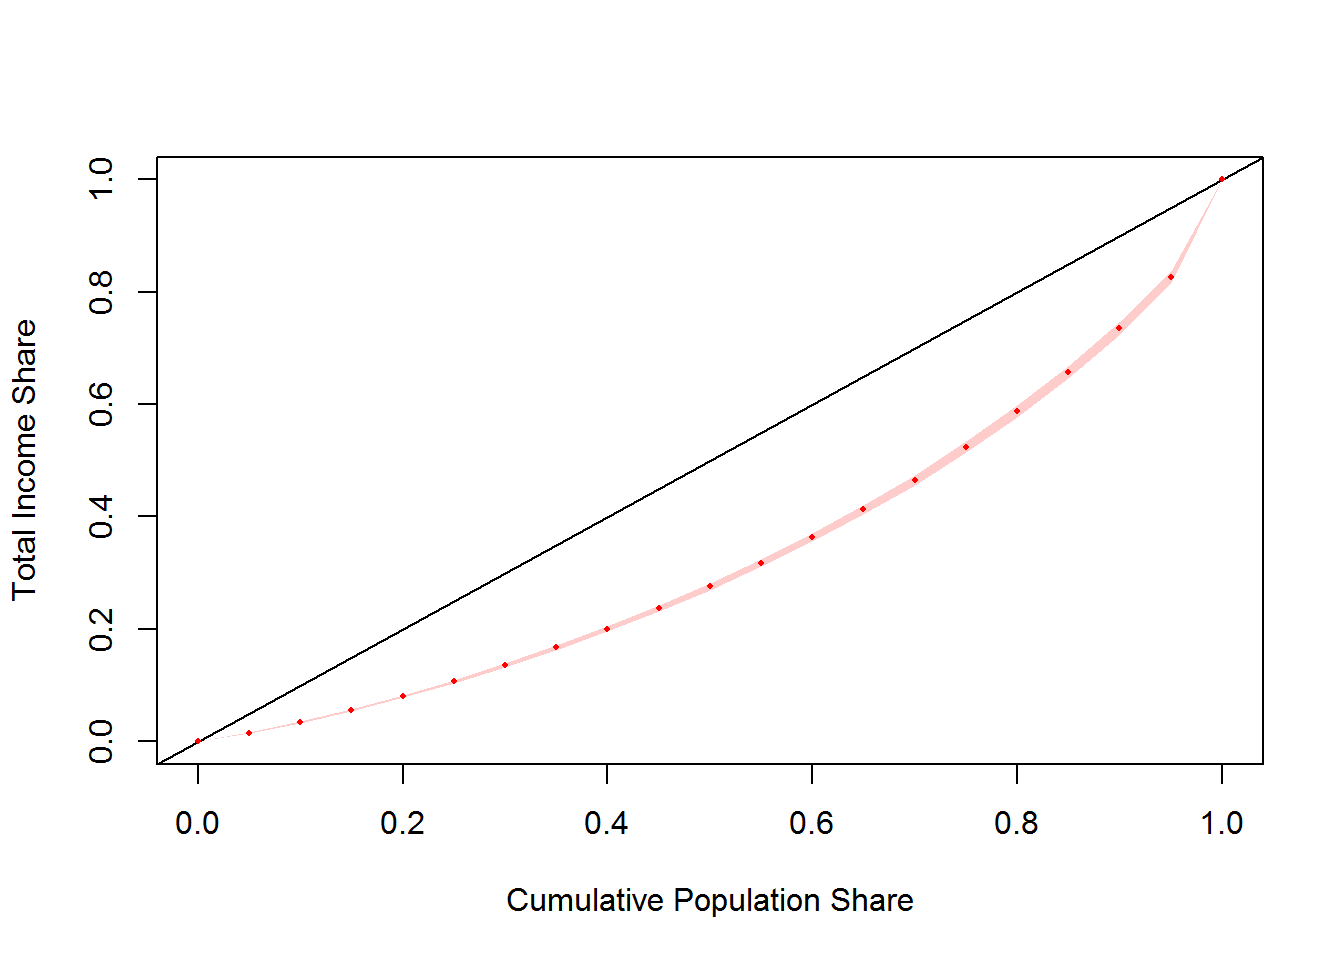
\includegraphics{context_files/figure-latex/unnamed-chunk-22-1.pdf}

\begin{Shaded}
\begin{Highlighting}[]
\CommentTok{# note: most survey commands in R use Inf degrees of freedom by default}
\CommentTok{# stata generally uses the degrees of freedom of the survey design.}
\CommentTok{# therefore, while this extended syntax serves to prove a precise replication of stata}
\CommentTok{# it is generally not necessary.}
\NormalTok{section_four_one <-}
\StringTok{    }\KeywordTok{data.frame}\NormalTok{( }
        \DataTypeTok{estimate =} \KeywordTok{coef}\NormalTok{( result.lin ) , }
        \DataTypeTok{standard_error =} \KeywordTok{SE}\NormalTok{( result.lin ) , }
        \DataTypeTok{ci_lower_bound =} 
            \KeywordTok{coef}\NormalTok{( result.lin ) +}\StringTok{ }
\StringTok{            }\KeywordTok{SE}\NormalTok{( result.lin ) *}\StringTok{ }
\StringTok{            }\KeywordTok{qt}\NormalTok{( }\FloatTok{0.025} \NormalTok{, }\KeywordTok{degf}\NormalTok{( }\KeywordTok{subset}\NormalTok{( des_nlsw88 , !}\KeywordTok{is.na}\NormalTok{( wage ) ) ) ) ,}
        \DataTypeTok{ci_upper_bound =} 
            \KeywordTok{coef}\NormalTok{( result.lin ) +}\StringTok{ }
\StringTok{            }\KeywordTok{SE}\NormalTok{( result.lin ) *}\StringTok{ }
\StringTok{            }\KeywordTok{qt}\NormalTok{( }\FloatTok{0.975} \NormalTok{, }\KeywordTok{degf}\NormalTok{( }\KeywordTok{subset}\NormalTok{( des_nlsw88 , !}\KeywordTok{is.na}\NormalTok{( wage ) ) ) )}
    \NormalTok{)}
    

\NormalTok{knitr::}\KeywordTok{kable}\NormalTok{(}
  \NormalTok{section_four_one , }\DataTypeTok{caption =} \StringTok{'Here is a nice table!'}\NormalTok{,}
  \DataTypeTok{booktabs =} \OtherTok{TRUE}
\NormalTok{)}
\end{Highlighting}
\end{Shaded}

\begin{table}

\caption{\label{tab:unnamed-chunk-22}Here is a nice table!}
\centering
\begin{tabular}[t]{lrrrr}
\toprule
  & estimate & standard\_error & ci\_lower\_bound & ci\_upper\_bound\\
\midrule
0 & 0.0000000 & 0.0000000 & 0.0000000 & 0.0000000\\
0.05 & 0.0151060 & 0.0004159 & 0.0142904 & 0.0159216\\
0.1 & 0.0342651 & 0.0007021 & 0.0328882 & 0.0356420\\
0.15 & 0.0558635 & 0.0010096 & 0.0538836 & 0.0578434\\
0.2 & 0.0801846 & 0.0014032 & 0.0774329 & 0.0829363\\
\addlinespace
0.25 & 0.1067687 & 0.0017315 & 0.1033732 & 0.1101642\\
0.3 & 0.1356307 & 0.0021301 & 0.1314535 & 0.1398078\\
0.35 & 0.1670287 & 0.0025182 & 0.1620903 & 0.1719670\\
0.4 & 0.2005501 & 0.0029161 & 0.1948315 & 0.2062687\\
0.45 & 0.2369209 & 0.0033267 & 0.2303971 & 0.2434447\\
\addlinespace
0.5 & 0.2759734 & 0.0037423 & 0.2686347 & 0.2833121\\
0.55 & 0.3180215 & 0.0041626 & 0.3098585 & 0.3261844\\
0.6 & 0.3633071 & 0.0045833 & 0.3543192 & 0.3722950\\
0.65 & 0.4125183 & 0.0050056 & 0.4027021 & 0.4223345\\
0.7 & 0.4657641 & 0.0054137 & 0.4551478 & 0.4763804\\
\addlinespace
0.75 & 0.5241784 & 0.0058003 & 0.5128039 & 0.5355529\\
0.8 & 0.5880894 & 0.0062464 & 0.5758401 & 0.6003388\\
0.85 & 0.6577051 & 0.0066148 & 0.6447333 & 0.6706769\\
0.9 & 0.7346412 & 0.0068289 & 0.7212497 & 0.7480328\\
0.95 & 0.8265786 & 0.0062686 & 0.8142857 & 0.8388715\\
1 & 1.0000000 & 0.0000000 & 1.0000000 & 1.0000000\\
\bottomrule
\end{tabular}
\end{table}

For additional usage examples of \texttt{svylorenz}, type
\texttt{?convey::svylorenz} in the R console.

\section{Gini index (svygini)}\label{gini-index-svygini}

The Gini index is an attempt to express the inequality presented in the
Lorenz curve as a single number. In essence, it is twice the area
between the equality curve and the real Lorenz curve. Put simply:

\[
\begin{aligned}
G &= 2 \bigg( \int_{0}^{1} pdp - \int_{0}^{1} L(p)dp \bigg) \\
\therefore G &= 1 - 2 \int_{0}^{1} L(p)dp
\end{aligned}
\]

where \(G=0\) in case of perfect equality and \(G = 1\) in the case of
perfect inequality.

The estimator proposed by \citep{osier2009} is defined as:

\[
\widehat{G} = \frac{ 2 \sum_{i \in S} w_i r_i y_i - \sum_{i \in S} w_i y_i }{ \hat{Y} }
\]

The linearized formula of \(\widehat{G}\) is used to calculate the SE.

\begin{center}\rule{0.5\linewidth}{\linethickness}\end{center}

\textbf{A replication example}

The R \texttt{vardpoor} package \citep{vardpoor}, created by researchers
at the Central Statistical Bureau of Latvia, includes a gini coefficient
calculation using the ultimate cluster method. The example below
reproduces those statistics.

Load and prepare the same data set:

\begin{Shaded}
\begin{Highlighting}[]
\CommentTok{# load the convey package}
\KeywordTok{library}\NormalTok{(convey)}

\CommentTok{# load the survey library}
\KeywordTok{library}\NormalTok{(survey)}

\CommentTok{# load the vardpoor library}
\KeywordTok{library}\NormalTok{(vardpoor)}

\CommentTok{# load the synthetic european union statistics on income & living conditions}
\KeywordTok{data}\NormalTok{(eusilc)}

\CommentTok{# make all column names lowercase}
\KeywordTok{names}\NormalTok{( eusilc ) <-}\StringTok{ }\KeywordTok{tolower}\NormalTok{( }\KeywordTok{names}\NormalTok{( eusilc ) )}

\CommentTok{# add a column with the row number}
\NormalTok{dati <-}\StringTok{ }\KeywordTok{data.table}\NormalTok{(}\DataTypeTok{IDd =} \DecValTok{1} \NormalTok{:}\StringTok{ }\KeywordTok{nrow}\NormalTok{(eusilc), eusilc)}

\CommentTok{# calculate the gini coefficient}
\CommentTok{# using the R vardpoor library}
\NormalTok{varpoord_gini_calculation <-}
\StringTok{    }\KeywordTok{varpoord}\NormalTok{(}
    
        \CommentTok{# analysis variable}
        \DataTypeTok{Y =} \StringTok{"eqincome"}\NormalTok{, }
        
        \CommentTok{# weights variable}
        \DataTypeTok{w_final =} \StringTok{"rb050"}\NormalTok{,}
        
        \CommentTok{# row number variable}
        \DataTypeTok{ID_level1 =} \StringTok{"IDd"}\NormalTok{,}
        
        \CommentTok{# strata variable}
        \DataTypeTok{H =} \StringTok{"db040"}\NormalTok{, }
        
        \DataTypeTok{N_h =} \OtherTok{NULL} \NormalTok{,}
        
        \CommentTok{# clustering variable}
        \DataTypeTok{PSU =} \StringTok{"rb030"}\NormalTok{, }
        
        \CommentTok{# data.table}
        \DataTypeTok{dataset =} \NormalTok{dati, }
        
        \CommentTok{# gini coefficient function}
        \DataTypeTok{type =} \StringTok{"lingini"}
        
    \NormalTok{)}

\CommentTok{# all calculations produced by vardpoor::lingini}
\NormalTok{varpoord_gini_calculation$all_result}
\end{Highlighting}
\end{Shaded}

\begin{verbatim}
##    type respondent_count n_nonzero pop_size    value value_eu        var
## 1: GINI            14827     14824  8182222 26.49652 26.48962 0.03783931
##           se         rse        cv absolute_margin_of_error
## 1: 0.1945233 0.007341467 0.7341467                0.3812587
##    relative_margin_of_error CI_lower CI_upper var_srs_HT var_cur_HT
## 1:                 1.438901 26.11526 26.87778 0.03660155 0.03783931
##    var_srs_ca deff_sam deff_est     deff
## 1: 0.03660155 1.033817        1 1.033817
\end{verbatim}

\begin{Shaded}
\begin{Highlighting}[]
\CommentTok{# construct a survey.design}
\CommentTok{# using our recommended setup}
\NormalTok{des_eusilc <-}\StringTok{ }
\StringTok{    }\KeywordTok{svydesign}\NormalTok{( }
        \DataTypeTok{ids =} \NormalTok{~}\StringTok{ }\NormalTok{rb030 , }
        \DataTypeTok{strata =} \NormalTok{~}\StringTok{ }\NormalTok{db040 ,  }
        \DataTypeTok{weights =} \NormalTok{~}\StringTok{ }\NormalTok{rb050 , }
        \DataTypeTok{data =} \NormalTok{eusilc}
    \NormalTok{)}

\CommentTok{# immediately run the convey_prep function on it}
\NormalTok{des_eusilc <-}\StringTok{ }\KeywordTok{convey_prep}\NormalTok{( des_eusilc )}

\CommentTok{# coefficients do match}
\NormalTok{varpoord_gini_calculation$all_result$value}
\end{Highlighting}
\end{Shaded}

\begin{verbatim}
## [1] 26.49652
\end{verbatim}

\begin{Shaded}
\begin{Highlighting}[]
\KeywordTok{coef}\NormalTok{( }\KeywordTok{svygini}\NormalTok{( ~}\StringTok{ }\NormalTok{eqincome , des_eusilc ) ) *}\StringTok{ }\DecValTok{100}
\end{Highlighting}
\end{Shaded}

\begin{verbatim}
## eqincome 
## 26.49652
\end{verbatim}

\begin{Shaded}
\begin{Highlighting}[]
\CommentTok{# variances do not match exactly}
\KeywordTok{attr}\NormalTok{( }\KeywordTok{svygini}\NormalTok{( ~}\StringTok{ }\NormalTok{eqincome , des_eusilc ) , }\StringTok{'var'} \NormalTok{) *}\StringTok{ }\DecValTok{10000}
\end{Highlighting}
\end{Shaded}

\begin{verbatim}
##            eqincome
## eqincome 0.03790739
\end{verbatim}

\begin{Shaded}
\begin{Highlighting}[]
\NormalTok{varpoord_gini_calculation$all_result$var}
\end{Highlighting}
\end{Shaded}

\begin{verbatim}
## [1] 0.03783931
\end{verbatim}

\begin{Shaded}
\begin{Highlighting}[]
\CommentTok{# standard errors do not match exactly}
\NormalTok{varpoord_gini_calculation$all_result$se}
\end{Highlighting}
\end{Shaded}

\begin{verbatim}
## [1] 0.1945233
\end{verbatim}

\begin{Shaded}
\begin{Highlighting}[]
\KeywordTok{SE}\NormalTok{( }\KeywordTok{svygini}\NormalTok{( ~}\StringTok{ }\NormalTok{eqincome , des_eusilc ) ) *}\StringTok{ }\DecValTok{100}
\end{Highlighting}
\end{Shaded}

\begin{verbatim}
##           eqincome
## eqincome 0.1946982
\end{verbatim}

By default, the \texttt{convey::svygini} function comes close to the
results of \texttt{vardpoor::lingini}. However, the measures of
uncertainty do not line up, because \texttt{library(vardpoor)} defaults
to the ultimate cluster method. This can be replicated with an
alternative setup of the \texttt{survey.design} object. The ultimate
cluster method is marginally less conservative, therefore, we do not
recommend using it as the default.

\begin{Shaded}
\begin{Highlighting}[]
\CommentTok{# within each strata, sum up the weights}
\NormalTok{cluster_sums <-}\StringTok{ }\KeywordTok{aggregate}\NormalTok{( eusilc$rb050 , }\KeywordTok{list}\NormalTok{( eusilc$db040 ) , sum )}

\CommentTok{# name the within-strata sums of weights the `cluster_sum`}
\KeywordTok{names}\NormalTok{( cluster_sums ) <-}\StringTok{ }\KeywordTok{c}\NormalTok{( }\StringTok{"db040"} \NormalTok{, }\StringTok{"cluster_sum"} \NormalTok{)}

\CommentTok{# merge this column back onto the data.frame}
\NormalTok{eusilc <-}\StringTok{ }\KeywordTok{merge}\NormalTok{( eusilc , cluster_sums )}

\CommentTok{# construct a survey.design}
\CommentTok{# with the fpc using the cluster sum}
\NormalTok{des_eusilc_ultimate_cluster <-}\StringTok{ }
\StringTok{    }\KeywordTok{svydesign}\NormalTok{( }
        \DataTypeTok{ids =} \NormalTok{~}\StringTok{ }\NormalTok{rb030 , }
        \DataTypeTok{strata =} \NormalTok{~}\StringTok{ }\NormalTok{db040 ,  }
        \DataTypeTok{weights =} \NormalTok{~}\StringTok{ }\NormalTok{rb050 , }
        \DataTypeTok{data =} \NormalTok{eusilc , }
        \DataTypeTok{fpc =} \NormalTok{~}\StringTok{ }\NormalTok{cluster_sum }
    \NormalTok{)}

\CommentTok{# again, immediately run the convey_prep function on the `survey.design`}
\NormalTok{des_eusilc_ultimate_cluster <-}\StringTok{ }\KeywordTok{convey_prep}\NormalTok{( des_eusilc_ultimate_cluster )}

\CommentTok{# matches}
\KeywordTok{attr}\NormalTok{( }\KeywordTok{svygini}\NormalTok{( ~}\StringTok{ }\NormalTok{eqincome , des_eusilc_ultimate_cluster ) , }\StringTok{'var'} \NormalTok{) *}\StringTok{ }\DecValTok{10000}
\end{Highlighting}
\end{Shaded}

\begin{verbatim}
##            eqincome
## eqincome 0.03783931
\end{verbatim}

\begin{Shaded}
\begin{Highlighting}[]
\NormalTok{varpoord_gini_calculation$all_result$var}
\end{Highlighting}
\end{Shaded}

\begin{verbatim}
## [1] 0.03783931
\end{verbatim}

\begin{Shaded}
\begin{Highlighting}[]
\CommentTok{# matches}
\NormalTok{varpoord_gini_calculation$all_result$se}
\end{Highlighting}
\end{Shaded}

\begin{verbatim}
## [1] 0.1945233
\end{verbatim}

\begin{Shaded}
\begin{Highlighting}[]
\KeywordTok{SE}\NormalTok{( }\KeywordTok{svygini}\NormalTok{( ~}\StringTok{ }\NormalTok{eqincome , des_eusilc_ultimate_cluster ) ) *}\StringTok{ }\DecValTok{100}
\end{Highlighting}
\end{Shaded}

\begin{verbatim}
##           eqincome
## eqincome 0.1945233
\end{verbatim}

For additional usage examples of \texttt{svygini}, type
\texttt{?convey::svygini} in the R console.

\section{Amato index (svyamato)}\label{amato-index-svyamato}

The Amato index is also based on the Lorenz curve, but instead of
focusing on the area of the curve, it focuses on its length.
\citep{arnold2012} proposes a formula not directly based in the Lorenz
curve, which \citep{barabesi2016} uses to present the following
estimator:

\[
\widehat{A} = \sum_{i \in S} w_i \bigg[ \frac{1}{\widehat{N}^2} + \frac{y_i^2}{\widehat{Y}^2} \bigg]^{\frac{1}{2}} \text{,}
\]

which also generates the linearized formula for SE estimation.

The minimum value \(A\) assumes is \(\sqrt{2}\) and the maximum is
\(2\). In order to get a measure in the interval \([0,1]\), the
standardized Amato index \(\widetilde{A}\) can be defined as:

\[
\widetilde{A} = \frac{ A - \sqrt{2} }{2 - \sqrt{2} } \text{ .}
\]

For additional usage examples of \texttt{svyamato}, type
\texttt{?convey::svyamato} in the R console.

\section{Zenga Index and Curve (svyzenga,
svyzengacurve)}\label{zenga-index-and-curve-svyzenga-svyzengacurve}

The Zenga index and its curve were proposed in \citep{zenga2007}. As
\citep{polisicchio2011} noticed, this curve derives directly from the
Lorenz curve, and can be defined as:

\[
Z(p) = 1 - \frac{L(p)}{p} \cdot \frac{1 - p}{1 - L(p)}.
\]

In the \texttt{convey} library, an experimental estimator based on the
Lorenz curve is used:

\[
\widehat{Z(p)} = \frac{ p \widehat{Y} - \widehat{\widetilde{Y}}(p) }{p \big[ \widehat{Y} - \widehat{\widetilde{Y}}(p) \big] }.
\]

In turn, the Zenga index derives from this curve and is defined as:

\[
Z = \int_0^1 Z(p)dp.
\]

However, its estimators were proposed by \citep{langel2012} and
\citep{barabesi2016}. In this library, the latter is used and is defined
as:

\[
\widehat{Z} = 1 - \sum_{i \in S} w_i \bigg[ \frac{ ( \widehat{N} - \widehat{H}_{y_i} ) ( \widehat{Y} -\widehat{K}_{y_i} ) }
{ \widehat{N} \cdot \widehat{H}_{y_i} \cdot \widehat{K}_{y_i} } \bigg]
\]

where \(\widehat{N}\) is the population total, \(\widehat{Y}\) is the
total income, \(\widehat{H}_{y_i}\) is the sum of incomes below or equal
to \(y_i\) and \(\widehat{N}_{y_i}\) is the sum of incomes greater or
equal to \(y_i\).

For additional usage examples of \texttt{svyzenga} or
\texttt{svyzengacurve}, type \texttt{?convey::svyzenga} or
\texttt{?convey::svyzengacurve} in the R console.

\section{Entropy-based Measures}\label{entropy-based-measures}

Entropy is a concept derived from information theory, meaning the
expected amount of information given the occurrence of an event.
Following \citep{shannon1948}, given an event \(y\) with probability
density function \(f(\cdot)\), the information content given the
occurrence of \(y\) can be defined as \(g(f(y)) \colon= - \log f(y)\).
Therefore, the expected information or, put simply, the \emph{entropy}
is

\[
H(f) \colon = -E \big[ \log f(y) \big] = - \int_{-\infty}^{\infty} f(y) \log f(y) dy
\]

Assuming a discrete distribution, with \(p_k\) as the probability of
occurring event \(k \in K\), the entropy formula takes the form:

\[
H = - \sum_{k \in K} p_k \log p_k \text{.}
\]

The main idea behind it is that the expected amount of information of an
event is inversely proportional to the probability of its occurrence. In
other words, the information derived from the observation of a rare
event is higher than of the information of more probable events.

Using the intuition presented in \citep{cowell2009}, substituting the
density function by the income share of an individual
\(s(q) = {F}^{-1}(q) / \int_{0}^{1} F^{-1}(t)dt = y/\mu\), the entropy
function becomes the Theil inequality index

\[
I_{Theil} = \int_{0}^{\infty} \frac{y}{\mu} \log \bigg( \frac{y}{\mu} \bigg) dF(y) = -H(s)
\]

Therefore, the entropy-based inequality measure increases as a person's
income \(y\) deviates from the mean \(\mu\). This is the basic idea
behind entropy-based inequality measures.

\section{Generalized Entropy and Decomposition (svygei,
svygeidec)}\label{generalized-entropy-and-decomposition-svygei-svygeidec}

Using a generalization of the information function, now defined as
\(g(f) = \frac{1}{\alpha-1} [ 1 - f^{\alpha - 1} ]\), the
\(\alpha\)-class entropy is \[
H_\alpha(f) = \frac{1}{\alpha - 1} \bigg[ 1 - \int_{-\infty}^{\infty} f(y)^{ \alpha - 1} f(y) dy \bigg] \text{.}
\]

This relates to a class of inequality measures, the Generalized entropy
indices, defined as:

\[
GE_\alpha = \frac{1}{\alpha^2 - \alpha} \int_{0}^\infty \bigg[ \bigg( \frac{y}{\mu} \bigg)^\alpha - 1 \bigg]dF(x) = - \frac{-H_\alpha(s) }{ \alpha } \text{.}
\]

The parameter \(\alpha\) also has an economic interpretation: as
\(\alpha\) increases, the influence of top incomes upon the index
increases. In some cases, this measure takes special forms, such as mean
log deviation and the aforementioned Theil index.

In order to estimate it, \citep{biewen2003} proposed the following:

\[
GE_\alpha =
\begin{cases}
( \alpha^2 - \alpha)^{-1} \big[ U_0^{\alpha - 1} U_1^{-\alpha} U_\alpha -1 \big], & \text{if } \alpha \in \mathbb{R} \setminus \{0,1\} \\
- T_0 U_0^{-1} + \log ( U_1 / U_0 ), &\text{if } \alpha \rightarrow 0 \\
T_1 U_1^{-1} - \log ( U_1 / U_0 ), & \text{if } \alpha \rightarrow 1
\end{cases}
\]

where \(U_\gamma = \sum_{i \in S} w_i \cdot y_i^\gamma\) and
\(T_\gamma = \sum_{i \in S} w_i \cdot y_i^\gamma \cdot \log y_i\). since
those are all functions of totals, the linearization of the indices are
easily achieved using the theorems described in \citep{deville1999}.

This class also has several desirable properties, such as additive
decomposition. The additive decomposition allows to compare the effects
of inequality within and between population groups on the population
inequality. Put simply, an additive decomposable index allows for:

\[
I_{Total} = I_{Between} + I_{Within} \text{.}
\]

\begin{center}\rule{0.5\linewidth}{\linethickness}\end{center}

\textbf{A replication example}

In July 2006, \citep{jenkins2006} presented at the North American Stata
Users' Group Meetings on the stata Generalized Entropy Index command.
The example below reproduces those statistics.

Load and prepare the same data set:

\begin{Shaded}
\begin{Highlighting}[]
\CommentTok{# load the convey package}
\KeywordTok{library}\NormalTok{(convey)}

\CommentTok{# load the survey library}
\KeywordTok{library}\NormalTok{(survey)}

\CommentTok{# load the foreign library}
\KeywordTok{library}\NormalTok{(foreign)}

\CommentTok{# create a temporary file on the local disk}
\NormalTok{tf <-}\StringTok{ }\KeywordTok{tempfile}\NormalTok{()}

\CommentTok{# store the location of the presentation file}
\NormalTok{presentation_zip <-}\StringTok{ "http://repec.org/nasug2006/nasug2006_jenkins.zip"}

\CommentTok{# download jenkins' presentation to the temporary file}
\KeywordTok{download.file}\NormalTok{( presentation_zip , tf , }\DataTypeTok{mode =} \StringTok{'wb'} \NormalTok{)}

\CommentTok{# unzip the contents of the archive}
\NormalTok{presentation_files <-}\StringTok{ }\KeywordTok{unzip}\NormalTok{( tf , }\DataTypeTok{exdir =} \KeywordTok{tempdir}\NormalTok{() )}

\CommentTok{# load the institute for fiscal studies' 1981, 1985, and 1991 data.frame objects}
\NormalTok{x81 <-}\StringTok{ }\KeywordTok{read.dta}\NormalTok{( }\KeywordTok{grep}\NormalTok{( }\StringTok{"ifs81"} \NormalTok{, presentation_files , }\DataTypeTok{value =} \OtherTok{TRUE} \NormalTok{) )}
\NormalTok{x85 <-}\StringTok{ }\KeywordTok{read.dta}\NormalTok{( }\KeywordTok{grep}\NormalTok{( }\StringTok{"ifs85"} \NormalTok{, presentation_files , }\DataTypeTok{value =} \OtherTok{TRUE} \NormalTok{) )}
\NormalTok{x91 <-}\StringTok{ }\KeywordTok{read.dta}\NormalTok{( }\KeywordTok{grep}\NormalTok{( }\StringTok{"ifs91"} \NormalTok{, presentation_files , }\DataTypeTok{value =} \OtherTok{TRUE} \NormalTok{) )}

\CommentTok{# stack each of these three years of data into a single data.frame}
\NormalTok{x <-}\StringTok{ }\KeywordTok{rbind}\NormalTok{( x81 , x85 , x91 )}
\end{Highlighting}
\end{Shaded}

Replicate the author's survey design statement from stata code..

\begin{verbatim}
. * account for clustering within HHs 
. version 8: svyset [pweight = wgt], psu(hrn)
pweight is wgt
psu is hrn
construct an
\end{verbatim}

.. into R code:

\begin{Shaded}
\begin{Highlighting}[]
\CommentTok{# initiate a linearized survey design object}
\NormalTok{y <-}\StringTok{ }\KeywordTok{svydesign}\NormalTok{( ~}\StringTok{ }\NormalTok{hrn , }\DataTypeTok{data =} \NormalTok{x , }\DataTypeTok{weights =} \NormalTok{~}\StringTok{ }\NormalTok{wgt )}

\CommentTok{# immediately run the `convey_prep` function on the survey design}
\NormalTok{z <-}\StringTok{ }\KeywordTok{convey_prep}\NormalTok{( y )}
\end{Highlighting}
\end{Shaded}

Replicate the author's subset statement and each of his svygei results..

\begin{verbatim}
. svygei x if year == 1981
 
Warning: x has 20 values = 0. Not used in calculations

Complex survey estimates of Generalized Entropy inequality indices
 
pweight: wgt                                   Number of obs    = 9752
Strata: <one>                                  Number of strata = 1
PSU: hrn                                       Number of PSUs   = 7459
                                               Population size  = 54766261
---------------------------------------------------------------------------
Index    |  Estimate   Std. Err.      z      P>|z|     [95% Conf. Interval]
---------+-----------------------------------------------------------------
GE(-1)   |  .1902062   .02474921     7.69    0.000      .1416987   .2387138
MLD      |  .1142851   .00275138    41.54    0.000      .1088925   .1196777
Theil    |  .1116923   .00226489    49.31    0.000      .1072532   .1161314
GE(2)    |   .128793   .00330774    38.94    0.000      .1223099    .135276
GE(3)    |  .1739994   .00662015    26.28    0.000      .1610242   .1869747
---------------------------------------------------------------------------
\end{verbatim}

..using R code:

\begin{Shaded}
\begin{Highlighting}[]
\NormalTok{z81 <-}\StringTok{ }\KeywordTok{subset}\NormalTok{( z , year ==}\StringTok{ }\DecValTok{1981} \NormalTok{)}

\KeywordTok{svygei}\NormalTok{( ~}\StringTok{ }\NormalTok{eybhc0 , }\KeywordTok{subset}\NormalTok{( z81 , eybhc0 >}\StringTok{ }\DecValTok{0} \NormalTok{) , }\DataTypeTok{epsilon =} \NormalTok{-}\DecValTok{1} \NormalTok{)}
\end{Highlighting}
\end{Shaded}

\begin{verbatim}
##            gei     SE
## eybhc0 0.19021 0.0247
\end{verbatim}

\begin{Shaded}
\begin{Highlighting}[]
\KeywordTok{svygei}\NormalTok{( ~}\StringTok{ }\NormalTok{eybhc0 , }\KeywordTok{subset}\NormalTok{( z81 , eybhc0 >}\StringTok{ }\DecValTok{0} \NormalTok{) , }\DataTypeTok{epsilon =} \DecValTok{0} \NormalTok{)}
\end{Highlighting}
\end{Shaded}

\begin{verbatim}
##            gei     SE
## eybhc0 0.11429 0.0028
\end{verbatim}

\begin{Shaded}
\begin{Highlighting}[]
\KeywordTok{svygei}\NormalTok{( ~}\StringTok{ }\NormalTok{eybhc0 , }\KeywordTok{subset}\NormalTok{( z81 , eybhc0 >}\StringTok{ }\DecValTok{0} \NormalTok{) )}
\end{Highlighting}
\end{Shaded}

\begin{verbatim}
##            gei     SE
## eybhc0 0.11169 0.0023
\end{verbatim}

\begin{Shaded}
\begin{Highlighting}[]
\KeywordTok{svygei}\NormalTok{( ~}\StringTok{ }\NormalTok{eybhc0 , }\KeywordTok{subset}\NormalTok{( z81 , eybhc0 >}\StringTok{ }\DecValTok{0} \NormalTok{) , }\DataTypeTok{epsilon =} \DecValTok{2} \NormalTok{)}
\end{Highlighting}
\end{Shaded}

\begin{verbatim}
##            gei     SE
## eybhc0 0.12879 0.0033
\end{verbatim}

\begin{Shaded}
\begin{Highlighting}[]
\KeywordTok{svygei}\NormalTok{( ~}\StringTok{ }\NormalTok{eybhc0 , }\KeywordTok{subset}\NormalTok{( z81 , eybhc0 >}\StringTok{ }\DecValTok{0} \NormalTok{) , }\DataTypeTok{epsilon =} \DecValTok{3} \NormalTok{)}
\end{Highlighting}
\end{Shaded}

\begin{verbatim}
##          gei     SE
## eybhc0 0.174 0.0066
\end{verbatim}

Confirm this replication applies for subsetted objects as well. Compare
stata output..

\begin{verbatim}
. svygei x if year == 1985 & x >= 1

Complex survey estimates of Generalized Entropy inequality indices
 
pweight: wgt                                   Number of obs    = 8969
Strata: <one>                                  Number of strata = 1
PSU: hrn                                       Number of PSUs   = 6950
                                               Population size  = 55042871
---------------------------------------------------------------------------
Index    |  Estimate   Std. Err.      z      P>|z|     [95% Conf. Interval]
---------+-----------------------------------------------------------------
GE(-1)   |  .1602358   .00936931    17.10    0.000      .1418723   .1785993
MLD      |   .127616   .00332187    38.42    0.000      .1211052   .1341267
Theil    |  .1337177   .00406302    32.91    0.000      .1257543    .141681
GE(2)    |  .1676393   .00730057    22.96    0.000      .1533304   .1819481
GE(3)    |  .2609507   .01850689    14.10    0.000      .2246779   .2972235
---------------------------------------------------------------------------
\end{verbatim}

..to R code:

\begin{Shaded}
\begin{Highlighting}[]
\NormalTok{z85 <-}\StringTok{ }\KeywordTok{subset}\NormalTok{( z , year ==}\StringTok{ }\DecValTok{1985} \NormalTok{)}

\KeywordTok{svygei}\NormalTok{( ~}\StringTok{ }\NormalTok{eybhc0 , }\KeywordTok{subset}\NormalTok{( z85 , eybhc0 >}\StringTok{ }\DecValTok{1} \NormalTok{) , }\DataTypeTok{epsilon =} \NormalTok{-}\DecValTok{1} \NormalTok{)}
\end{Highlighting}
\end{Shaded}

\begin{verbatim}
##            gei     SE
## eybhc0 0.16024 0.0094
\end{verbatim}

\begin{Shaded}
\begin{Highlighting}[]
\KeywordTok{svygei}\NormalTok{( ~}\StringTok{ }\NormalTok{eybhc0 , }\KeywordTok{subset}\NormalTok{( z85 , eybhc0 >}\StringTok{ }\DecValTok{1} \NormalTok{) , }\DataTypeTok{epsilon =} \DecValTok{0} \NormalTok{)}
\end{Highlighting}
\end{Shaded}

\begin{verbatim}
##            gei     SE
## eybhc0 0.12762 0.0033
\end{verbatim}

\begin{Shaded}
\begin{Highlighting}[]
\KeywordTok{svygei}\NormalTok{( ~}\StringTok{ }\NormalTok{eybhc0 , }\KeywordTok{subset}\NormalTok{( z85 , eybhc0 >}\StringTok{ }\DecValTok{1} \NormalTok{) )}
\end{Highlighting}
\end{Shaded}

\begin{verbatim}
##            gei     SE
## eybhc0 0.13372 0.0041
\end{verbatim}

\begin{Shaded}
\begin{Highlighting}[]
\KeywordTok{svygei}\NormalTok{( ~}\StringTok{ }\NormalTok{eybhc0 , }\KeywordTok{subset}\NormalTok{( z85 , eybhc0 >}\StringTok{ }\DecValTok{1} \NormalTok{) , }\DataTypeTok{epsilon =} \DecValTok{2} \NormalTok{)}
\end{Highlighting}
\end{Shaded}

\begin{verbatim}
##            gei     SE
## eybhc0 0.16764 0.0073
\end{verbatim}

\begin{Shaded}
\begin{Highlighting}[]
\KeywordTok{svygei}\NormalTok{( ~}\StringTok{ }\NormalTok{eybhc0 , }\KeywordTok{subset}\NormalTok{( z85 , eybhc0 >}\StringTok{ }\DecValTok{1} \NormalTok{) , }\DataTypeTok{epsilon =} \DecValTok{3} \NormalTok{)}
\end{Highlighting}
\end{Shaded}

\begin{verbatim}
##            gei     SE
## eybhc0 0.26095 0.0185
\end{verbatim}

For additional usage examples of \texttt{svygei} or \texttt{svygeidec},
type \texttt{?convey::svygei} or \texttt{?convey::svygeidec} in the R
console.

\section{Rényi Divergence (svyrenyi)}\label{renyi-divergence-svyrenyi}

Another measure used in areas like ecology, statistics and information
theory is Rényi divergence measure. Using the formula defined in
\citep{langel2012}, the estimator can be defined as:

\[
\widehat{R}_\alpha =
\begin{cases}
\frac{1}{\alpha - 1} \log \bigg[ \widehat{N}^{\alpha - 1} \sum_{i \in S} w_i \cdot \bigg( \frac{y_k}{ \widehat{Y} } \bigg) \bigg], &\text{if } \alpha \neq 1, \\
\sum_{i \in S} \frac{w_i y_i}{ \widehat{Y}} \log \frac{\widehat{N} y_i}{\widehat{Y}}, &\text{if } \alpha = 1,
\end{cases}
\]

where \(\alpha\) is a parameter with a similar economic interpretation
to that of the \(GE_\alpha\) index.

For additional usage examples of \texttt{svyrenyi}, type
\texttt{?convey::svyrenyi} in the R console.

\section{J-Divergence and Decomposition (svyjdiv,
svyjdivdec)}\label{j-divergence-and-decomposition-svyjdiv-svyjdivdec}

Proposed by \citep{rohde2016}, the J-divergence measure can be seen as
the sum of \(GE_0\) and \(GE_1\), satisfying axioms that, individually,
those two indices do not. Using \(U_\gamma\) and \(T_\gamma\) functions
defined in \ref{subsection.3.3.1}, the estimator can be defined as:

\[
\begin{aligned}
\widehat{J} &= \frac{1}{\widehat{N}} \sum_{i \in S} w_i \bigg( \frac{ y_i - \widehat{\mu} }{ \widehat{\mu} } \bigg) \log \bigg( \frac{y_i}{\widehat{\mu}} \bigg) \\
\therefore \widehat{J} &= \frac{\widehat{T}_1}{\widehat{U}_1} - \frac{ \widehat{T}_0 }{ \widehat{U}_0 }
\end{aligned}
\]

Since it is a sum of two additive decomposable measures, \(J\) itself is
decomposable.

For additional usage examples of \texttt{svyjdiv} or
\texttt{svyjdivdec}, type \texttt{?convey::svyjdiv} or
\texttt{?convey::svyjdivdec} in the R console.

\section{Atkinson index (svyatk)}\label{atkinson-index-svyatk}

Although the original formula was proposed in \citep{atkinson1970}, the
estimator used here comes from \citep{biewen2003}:

\[
\widehat{A}_\epsilon =
\begin{cases}
 1 - \widehat{U}_0^{ - \epsilon/(1 - \epsilon) } \widehat{U}_1^{ -1 } \widehat{U}_{1 - \epsilon}^{ 1/(1 - \epsilon) } , &\text{if } \epsilon \in \mathbb{R}_+ \setminus\{ 1 \} \\
1 - \widehat{U}_0 \widehat{U}_0^{-1} exp( \widehat{T}_0 \widehat{U}_0^{-1} ), &\text{if } \epsilon \rightarrow1
\end{cases}
\]

The \(\epsilon\) is an inequality aversion parameter: as it approaches
infinity, more weight is given to incomes in bottom of the distribution.

\begin{center}\rule{0.5\linewidth}{\linethickness}\end{center}

\textbf{A replication example}

In July 2006, \citep{jenkins2006} presented at the North American Stata
Users' Group Meetings on the stata Atkinson Index command. The example
below reproduces those statistics.

Load and prepare the same data set:

\begin{Shaded}
\begin{Highlighting}[]
\CommentTok{# load the convey package}
\KeywordTok{library}\NormalTok{(convey)}

\CommentTok{# load the survey library}
\KeywordTok{library}\NormalTok{(survey)}

\CommentTok{# load the foreign library}
\KeywordTok{library}\NormalTok{(foreign)}

\CommentTok{# create a temporary file on the local disk}
\NormalTok{tf <-}\StringTok{ }\KeywordTok{tempfile}\NormalTok{()}

\CommentTok{# store the location of the presentation file}
\NormalTok{presentation_zip <-}\StringTok{ "http://repec.org/nasug2006/nasug2006_jenkins.zip"}

\CommentTok{# download jenkins' presentation to the temporary file}
\KeywordTok{download.file}\NormalTok{( presentation_zip , tf , }\DataTypeTok{mode =} \StringTok{'wb'} \NormalTok{)}

\CommentTok{# unzip the contents of the archive}
\NormalTok{presentation_files <-}\StringTok{ }\KeywordTok{unzip}\NormalTok{( tf , }\DataTypeTok{exdir =} \KeywordTok{tempdir}\NormalTok{() )}

\CommentTok{# load the institute for fiscal studies' 1981, 1985, and 1991 data.frame objects}
\NormalTok{x81 <-}\StringTok{ }\KeywordTok{read.dta}\NormalTok{( }\KeywordTok{grep}\NormalTok{( }\StringTok{"ifs81"} \NormalTok{, presentation_files , }\DataTypeTok{value =} \OtherTok{TRUE} \NormalTok{) )}
\NormalTok{x85 <-}\StringTok{ }\KeywordTok{read.dta}\NormalTok{( }\KeywordTok{grep}\NormalTok{( }\StringTok{"ifs85"} \NormalTok{, presentation_files , }\DataTypeTok{value =} \OtherTok{TRUE} \NormalTok{) )}
\NormalTok{x91 <-}\StringTok{ }\KeywordTok{read.dta}\NormalTok{( }\KeywordTok{grep}\NormalTok{( }\StringTok{"ifs91"} \NormalTok{, presentation_files , }\DataTypeTok{value =} \OtherTok{TRUE} \NormalTok{) )}

\CommentTok{# stack each of these three years of data into a single data.frame}
\NormalTok{x <-}\StringTok{ }\KeywordTok{rbind}\NormalTok{( x81 , x85 , x91 )}
\end{Highlighting}
\end{Shaded}

Replicate the author's survey design statement from stata code..

\begin{verbatim}
. * account for clustering within HHs 
. version 8: svyset [pweight = wgt], psu(hrn)
pweight is wgt
psu is hrn
construct an
\end{verbatim}

.. into R code:

\begin{Shaded}
\begin{Highlighting}[]
\CommentTok{# initiate a linearized survey design object}
\NormalTok{y <-}\StringTok{ }\KeywordTok{svydesign}\NormalTok{( ~}\StringTok{ }\NormalTok{hrn , }\DataTypeTok{data =} \NormalTok{x , }\DataTypeTok{weights =} \NormalTok{~}\StringTok{ }\NormalTok{wgt )}

\CommentTok{# immediately run the `convey_prep` function on the survey design}
\NormalTok{z <-}\StringTok{ }\KeywordTok{convey_prep}\NormalTok{( y )}
\end{Highlighting}
\end{Shaded}

Replicate the author's subset statement and each of his svyatk results
with stata..

\begin{verbatim}
. svyatk x if year == 1981
 
Warning: x has 20 values = 0. Not used in calculations

Complex survey estimates of Atkinson inequality indices
 
pweight: wgt                                   Number of obs    = 9752
Strata: <one>                                  Number of strata = 1
PSU: hrn                                       Number of PSUs   = 7459
                                               Population size  = 54766261
---------------------------------------------------------------------------
Index    |  Estimate   Std. Err.      z      P>|z|     [95% Conf. Interval]
---------+-----------------------------------------------------------------
A(0.5)   |  .0543239   .00107583    50.49    0.000      .0522153   .0564324
A(1)     |  .1079964   .00245424    44.00    0.000      .1031862   .1128066
A(1.5)   |  .1701794   .0066943    25.42    0.000       .1570588      .1833
A(2)     |  .2755788   .02597608    10.61    0.000      .2246666    .326491
A(2.5)   |  .4992701   .06754311     7.39    0.000       .366888   .6316522
---------------------------------------------------------------------------
\end{verbatim}

..using R code:

\begin{Shaded}
\begin{Highlighting}[]
\NormalTok{z81 <-}\StringTok{ }\KeywordTok{subset}\NormalTok{( z , year ==}\StringTok{ }\DecValTok{1981} \NormalTok{)}

\KeywordTok{svyatk}\NormalTok{( ~}\StringTok{ }\NormalTok{eybhc0 , }\KeywordTok{subset}\NormalTok{( z81 , eybhc0 >}\StringTok{ }\DecValTok{0} \NormalTok{) , }\DataTypeTok{epsilon =} \FloatTok{0.5} \NormalTok{)}
\end{Highlighting}
\end{Shaded}

\begin{verbatim}
##        atkinson     SE
## eybhc0 0.054324 0.0011
\end{verbatim}

\begin{Shaded}
\begin{Highlighting}[]
\KeywordTok{svyatk}\NormalTok{( ~}\StringTok{ }\NormalTok{eybhc0 , }\KeywordTok{subset}\NormalTok{( z81 , eybhc0 >}\StringTok{ }\DecValTok{0} \NormalTok{) )}
\end{Highlighting}
\end{Shaded}

\begin{verbatim}
##        atkinson     SE
## eybhc0    0.108 0.0025
\end{verbatim}

\begin{Shaded}
\begin{Highlighting}[]
\KeywordTok{svyatk}\NormalTok{( ~}\StringTok{ }\NormalTok{eybhc0 , }\KeywordTok{subset}\NormalTok{( z81 , eybhc0 >}\StringTok{ }\DecValTok{0} \NormalTok{) , }\DataTypeTok{epsilon =} \FloatTok{1.5} \NormalTok{)}
\end{Highlighting}
\end{Shaded}

\begin{verbatim}
##        atkinson     SE
## eybhc0  0.17018 0.0067
\end{verbatim}

\begin{Shaded}
\begin{Highlighting}[]
\KeywordTok{svyatk}\NormalTok{( ~}\StringTok{ }\NormalTok{eybhc0 , }\KeywordTok{subset}\NormalTok{( z81 , eybhc0 >}\StringTok{ }\DecValTok{0} \NormalTok{) , }\DataTypeTok{epsilon =} \DecValTok{2} \NormalTok{)}
\end{Highlighting}
\end{Shaded}

\begin{verbatim}
##        atkinson    SE
## eybhc0  0.27558 0.026
\end{verbatim}

\begin{Shaded}
\begin{Highlighting}[]
\KeywordTok{svyatk}\NormalTok{( ~}\StringTok{ }\NormalTok{eybhc0 , }\KeywordTok{subset}\NormalTok{( z81 , eybhc0 >}\StringTok{ }\DecValTok{0} \NormalTok{) , }\DataTypeTok{epsilon =} \FloatTok{2.5} \NormalTok{)}
\end{Highlighting}
\end{Shaded}

\begin{verbatim}
##        atkinson     SE
## eybhc0  0.49927 0.0675
\end{verbatim}

Confirm this replication applies for subsetted objects as well,
comparing stata code..

\begin{verbatim}
. svyatk x if year == 1981 & x >= 1

Complex survey estimates of Atkinson inequality indices
 
pweight: wgt                                   Number of obs    = 9748
Strata: <one>                                  Number of strata = 1
PSU: hrn                                       Number of PSUs   = 7457
                                               Population size  = 54744234
---------------------------------------------------------------------------
Index    |  Estimate   Std. Err.      z      P>|z|     [95% Conf. Interval]
---------+-----------------------------------------------------------------
A(0.5)   |  .0540059   .00105011    51.43    0.000      .0519477   .0560641
A(1)     |  .1066082   .00223318    47.74    0.000      .1022313   .1109852
A(1.5)   |  .1638299   .00483069    33.91    0.000       .154362   .1732979
A(2)     |  .2443206   .01425258    17.14    0.000      .2163861   .2722552
A(2.5)   |   .394787   .04155221     9.50    0.000      .3133461   .4762278
---------------------------------------------------------------------------
\end{verbatim}

..to R code:

\begin{Shaded}
\begin{Highlighting}[]
\NormalTok{z81_two <-}\StringTok{ }\KeywordTok{subset}\NormalTok{( z , year ==}\StringTok{ }\DecValTok{1981} \NormalTok{&}\StringTok{ }\NormalTok{eybhc0 >}\StringTok{ }\DecValTok{1} \NormalTok{)}

\KeywordTok{svyatk}\NormalTok{( ~}\StringTok{ }\NormalTok{eybhc0 , z81_two , }\DataTypeTok{epsilon =} \FloatTok{0.5} \NormalTok{)}
\end{Highlighting}
\end{Shaded}

\begin{verbatim}
##        atkinson     SE
## eybhc0 0.054006 0.0011
\end{verbatim}

\begin{Shaded}
\begin{Highlighting}[]
\KeywordTok{svyatk}\NormalTok{( ~}\StringTok{ }\NormalTok{eybhc0 , z81_two )}
\end{Highlighting}
\end{Shaded}

\begin{verbatim}
##        atkinson     SE
## eybhc0  0.10661 0.0022
\end{verbatim}

\begin{Shaded}
\begin{Highlighting}[]
\KeywordTok{svyatk}\NormalTok{( ~}\StringTok{ }\NormalTok{eybhc0 , z81_two , }\DataTypeTok{epsilon =} \FloatTok{1.5} \NormalTok{)}
\end{Highlighting}
\end{Shaded}

\begin{verbatim}
##        atkinson     SE
## eybhc0  0.16383 0.0048
\end{verbatim}

\begin{Shaded}
\begin{Highlighting}[]
\KeywordTok{svyatk}\NormalTok{( ~}\StringTok{ }\NormalTok{eybhc0 , z81_two , }\DataTypeTok{epsilon =} \DecValTok{2} \NormalTok{)}
\end{Highlighting}
\end{Shaded}

\begin{verbatim}
##        atkinson     SE
## eybhc0  0.24432 0.0143
\end{verbatim}

\begin{Shaded}
\begin{Highlighting}[]
\KeywordTok{svyatk}\NormalTok{( ~}\StringTok{ }\NormalTok{eybhc0 , z81_two , }\DataTypeTok{epsilon =} \FloatTok{2.5} \NormalTok{)}
\end{Highlighting}
\end{Shaded}

\begin{verbatim}
##        atkinson     SE
## eybhc0  0.39479 0.0416
\end{verbatim}

For additional usage examples of \texttt{svyatk}, type
\texttt{?convey::svyatk} in the R console.

\chapter{Wellbeing Measures}\label{wellbeing}

djalmapessoa\_look do any of the other functions need to be moved to
this wellbeing chapter?

\section{The Gender Pay Gap (svygpg)}\label{the-gender-pay-gap-svygpg}

For additional usage examples of \texttt{svygpg}, type
\texttt{?convey::svygpg} in the R console.

here are the references

\citep{osier2009} and \citep{deville1999}

\section{Quintile Share Ratio
(svyqsr)}\label{quintile-share-ratio-svyqsr}

For additional usage examples of \texttt{svyqsr}, type
\texttt{?convey::svyqsr} in the R console.

here are the references

\citep{osier2009} and \citep{deville1999}

\chapter{Multidimensional Indices}\label{multidimensional}

Inequality and poverty can be seen as multidimensional concepts,
combining several livelihood characteristics. Usual approaches take into
account income, housing, sanitation, etc.

In order to transform these different measures from into meaningful
numbers, economic theory builds on the idea of utility functions.
Utility is a measure of well-being, assigning a ``well-being score'' to
a vector of characteristics. Depending on the utility function, the
analyst may allow for substitutions among characteristics: for instance,
someone with a slightly lower income, but with access to sanitation, can
have a higher wellbeing than someone with a higher income, but without
access to sanitation. This depends on the set of weights given to the
set of attributes.

Most measures below follow from this kind of two-step procedure: (1)
estimating individual scores from an individual's set of
characteristics; then (2) aggregating those individual scores into a
single measure for the population.

The following section will present a measure of multidimensional poverty
and a measure of multidimensional inequality, describing the main
aspects of the theory and estimation procedures of each.

\section{Alkire-Foster Class and Decomposition (svyafc,
svyafcdec)}\label{alkire-foster-class-and-decomposition-svyafc-svyafcdec}

This class of measures are defined in \citep{alkire2011}, using what is
called the ``dual cutoff'' approach. This method applies a cutoffs to
define dimensional deprivations and another cutoff for multidimensional
deprivation.

To analyze a population of \(n\) individuals across \(d\) achievement
dimensions, the first step of the method is applying a FGT-like
transformation to each dimension, defined as

\[
g_{ij}^\alpha = \bigg( \frac{ z_j - x_{ij} }{ z_j } \bigg)^{\alpha}
\]

where \(i\) is an observation index, \(j\) is a dimension index and
\(\alpha\) is an exponent weighting the deprivation intensity. If
\(\alpha=0\), then \(g_{ij}^0\) becomes a binary variable, assuming
value \(1\) if person \(i\) is deprived in dimension \(j\) and \(0\)
otherwise. The \(n \times d\) matrix \(G^\alpha\) will be referred to as
\emph{deprivation matrix}.

Each dimension receives a weight \(w_j\), so that the weighted sum of
multidimensional deprivation is the matrix multiplication of
\(G^\alpha\) by the \(j \times 1\) vector \(W = [w_j]\). The
\(n \times 1\) vector \(C^\alpha = [c^\alpha_i]\) is the weighted sum of
dimensional deprivation scores, i.e.,

\[
c^\alpha_{i} = \sum_{j \in d} w_j g_{ij}^\alpha
\]

The second cutoff is defining those considered to be multidimensionally
poor. Assuming that \(\sum_{j \in d} w_j = 1\), the multidimensional
cutoff \(k\) belongs to the interval \((0,1]\). If
\(c^0_{i} \geqslant k\), then this person is considered
multidimensionally poor. The \emph{censored vector of deprivation sums}
\(C^\alpha(k)\) is defined as

\[
C^\alpha (k) = \bigg[ c_{ij}^\alpha \cdot \delta \big( c_{ij}^0 \geqslant k \big) \bigg] \text{,}
\]

where \(\delta(A)\) is an indicator function, taking value \(1\) if
condition \(A\) is true and \(0\) otherwise. If
\(k \geqslant \min{ w_j }\), this is called the ``union approach'',
where a person is considered poor if she is poor in at least one
dimension. On the other extreme, the ``intersection approach'' happens
when \(k = 1\), meaning that a person is considered poor if she is poor
in all dimensions.

The average of vector \(C^0 (k)\) returns the multidimensional headcount
ratio. For the multidimensional FGT class, a general measure can be
defined as

\[
M^\alpha = \frac{1}{n} \sum_{i \in n} \sum_{j \in d} w_j g_{ij}^{\alpha}(k) \text{, } \alpha \geq 0 \text{,}
\]

where
\(g_{ij}^{\alpha}(k) = g_{ij}^\alpha \cdot \delta \big( c^0_i \geqslant k \big)\).

For inferential purposes, since this variable is actually the average of
scores \(\sum_{j \in d} w_j g_{ij}^{\alpha}(k)\), the linearization is
straightforward.

\subsection{Dimensional and group
decomposition}\label{dimensional-and-group-decomposition}

{[}start with dimensional{]}

\begin{center}\rule{0.5\linewidth}{\linethickness}\end{center}

\textbf{A replication example}

In November 2015, Christopher Jindra presented at the Oxford Poverty and
Human Development Initiative on the Alkire-Foster multidimensional
poverty measure. His presentation can be viewed
\href{http://www.ophi.org.uk/wp-content/uploads/Jindra_151109_OPHISeminar.pdf}{here}.
The example below reproduces those statistics.

Load and prepare the same data set:

\begin{Shaded}
\begin{Highlighting}[]
\CommentTok{# load the convey package}
\KeywordTok{library}\NormalTok{(convey)}

\CommentTok{# load the survey library}
\KeywordTok{library}\NormalTok{(survey)}

\CommentTok{# load the stata-style webuse library}
\KeywordTok{library}\NormalTok{(webuse)}

\CommentTok{# load the same microdata set used by Jindra in his presentation}
\KeywordTok{webuse}\NormalTok{(}\StringTok{"nlsw88"}\NormalTok{)}

\CommentTok{# coerce that `tbl_df` to a standard R `data.frame`}
\NormalTok{nlsw88 <-}\StringTok{ }\KeywordTok{data.frame}\NormalTok{( nlsw88 )}

\CommentTok{# create a `collgrad` column}
\NormalTok{nlsw88$collgrad <-}
\StringTok{    }\KeywordTok{factor}\NormalTok{( }
        \KeywordTok{as.numeric}\NormalTok{( nlsw88$collgrad ) , }
        \DataTypeTok{label =} \KeywordTok{c}\NormalTok{( }\StringTok{'not college grad'} \NormalTok{, }\StringTok{'college grad'} \NormalTok{) , }
        \DataTypeTok{ordered =} \OtherTok{TRUE} 
      \NormalTok{)}

\CommentTok{# initiate a linearized survey design object}
\NormalTok{des_nlsw88 <-}\StringTok{ }\KeywordTok{svydesign}\NormalTok{( }\DataTypeTok{ids =} \NormalTok{~}\DecValTok{1} \NormalTok{, }\DataTypeTok{data =} \NormalTok{nlsw88 )}

\CommentTok{# immediately run the `convey_prep` function on the survey design}
\NormalTok{des_nlsw88 <-}\StringTok{ }\KeywordTok{convey_prep}\NormalTok{(des_nlsw88)}
\end{Highlighting}
\end{Shaded}

Replicate PDF page 9

\begin{Shaded}
\begin{Highlighting}[]
\NormalTok{page_nine <-}
\StringTok{  }\KeywordTok{svyafc}\NormalTok{(}
    \NormalTok{~}\StringTok{ }\NormalTok{wage +}\StringTok{ }\NormalTok{collgrad +}\StringTok{ }\NormalTok{hours , }
    \DataTypeTok{design =} \NormalTok{des_nlsw88 , }
    \DataTypeTok{cutoffs =} \KeywordTok{list}\NormalTok{( }\DecValTok{4}\NormalTok{, }\StringTok{'college grad'} \NormalTok{, }\DecValTok{26} \NormalTok{) , }
    \DataTypeTok{k =} \DecValTok{1}\NormalTok{/}\DecValTok{3} \NormalTok{, }\DataTypeTok{g =} \DecValTok{0} \NormalTok{, }
    \DataTypeTok{na.rm =} \OtherTok{TRUE}
  \NormalTok{)}

\CommentTok{# MO and seMO}
\KeywordTok{print}\NormalTok{( page_nine )}
\end{Highlighting}
\end{Shaded}

\begin{verbatim}
##      alkire-foster     SE
## [1,]       0.36991 0.0053
\end{verbatim}

\begin{Shaded}
\begin{Highlighting}[]
\CommentTok{# H seH and A seA}
\KeywordTok{print}\NormalTok{( }\KeywordTok{attr}\NormalTok{( page_nine , }\StringTok{"extra"} \NormalTok{) )}
\end{Highlighting}
\end{Shaded}

\begin{verbatim}
##        coef          SE
## H 0.8082070 0.008316807
## A 0.4576895 0.004573443
\end{verbatim}

Replicate PDF page 10

\begin{Shaded}
\begin{Highlighting}[]
\NormalTok{page_ten <-}\StringTok{ }\OtherTok{NULL}

\CommentTok{# loop through every poverty cutoff `k`}
\NormalTok{for( ks in }\KeywordTok{seq}\NormalTok{( }\FloatTok{0.1} \NormalTok{, }\DecValTok{1} \NormalTok{, .}\DecValTok{1} \NormalTok{) )\{}
    
    \NormalTok{this_ks <-}
\StringTok{        }\KeywordTok{svyafc}\NormalTok{(}
            \NormalTok{~}\StringTok{ }\NormalTok{wage +}\StringTok{ }\NormalTok{collgrad +}\StringTok{ }\NormalTok{hours , }
            \DataTypeTok{design =} \NormalTok{des_nlsw88 , }
            \DataTypeTok{cutoffs =} \KeywordTok{list}\NormalTok{( }\DecValTok{4} \NormalTok{, }\StringTok{'college grad'} \NormalTok{, }\DecValTok{26} \NormalTok{) , }
            \DataTypeTok{k =} \NormalTok{ks , }
            \DataTypeTok{g =} \DecValTok{0} \NormalTok{, }
            \DataTypeTok{na.rm =} \OtherTok{TRUE} 
           \NormalTok{)}
    
    \NormalTok{page_ten <-}
\StringTok{        }\KeywordTok{rbind}\NormalTok{(}
            \NormalTok{page_ten ,}
            \KeywordTok{data.frame}\NormalTok{( }
                \DataTypeTok{k =} \NormalTok{ks , }
                \DataTypeTok{MO =} \KeywordTok{coef}\NormalTok{( this_ks ) ,}
                \DataTypeTok{seMO =} \KeywordTok{SE}\NormalTok{( this_ks ) ,}
                \DataTypeTok{H =} \KeywordTok{attr}\NormalTok{( this_ks , }\StringTok{"extra"} \NormalTok{)[ }\DecValTok{1} \NormalTok{, }\DecValTok{1} \NormalTok{] ,}
                \DataTypeTok{seH =} \KeywordTok{attr}\NormalTok{( this_ks , }\StringTok{"extra"} \NormalTok{)[ }\DecValTok{1} \NormalTok{, }\DecValTok{2} \NormalTok{] ,}
                \DataTypeTok{A =} \KeywordTok{attr}\NormalTok{( this_ks , }\StringTok{"extra"} \NormalTok{)[ }\DecValTok{2} \NormalTok{, }\DecValTok{1} \NormalTok{] ,}
                \DataTypeTok{seA =} \KeywordTok{attr}\NormalTok{( this_ks , }\StringTok{"extra"} \NormalTok{)[ }\DecValTok{2} \NormalTok{, }\DecValTok{2} \NormalTok{]}
          \NormalTok{)}
        \NormalTok{)}
    
\NormalTok{\}}

\NormalTok{knitr::}\KeywordTok{kable}\NormalTok{(}
  \NormalTok{page_ten , }\DataTypeTok{caption =} \StringTok{'Here is a nice table!'}\NormalTok{,}
  \DataTypeTok{booktabs =} \OtherTok{TRUE}
\NormalTok{)}
\end{Highlighting}
\end{Shaded}

\begin{table}

\caption{\label{tab:unnamed-chunk-41}Here is a nice table!}
\centering
\begin{tabular}[t]{rrrrrrr}
\toprule
k & MO & seMO & H & seH & A & seA\\
\midrule
0.1 & 0.3699078 & 0.0053059 & 0.8082070 & 0.0083168 & 0.4576895 & 0.0045734\\
0.2 & 0.3699078 & 0.0053059 & 0.8082070 & 0.0083168 & 0.4576895 & 0.0045734\\
0.3 & 0.3699078 & 0.0053059 & 0.8082070 & 0.0083168 & 0.4576895 & 0.0045734\\
0.4 & 0.1865894 & 0.0068123 & 0.2582516 & 0.0092455 & 0.7225101 & 0.0051745\\
0.5 & 0.1865894 & 0.0068123 & 0.2582516 & 0.0092455 & 0.7225101 & 0.0051745\\
\addlinespace
0.6 & 0.1865894 & 0.0068123 & 0.2582516 & 0.0092455 & 0.7225101 & 0.0051745\\
0.7 & 0.0432649 & 0.0042978 & 0.0432649 & 0.0042978 & 1.0000000 & 0.0000000\\
0.8 & 0.0432649 & 0.0042978 & 0.0432649 & 0.0042978 & 1.0000000 & 0.0000000\\
0.9 & 0.0432649 & 0.0042978 & 0.0432649 & 0.0042978 & 1.0000000 & 0.0000000\\
1.0 & 0.0432649 & 0.0042978 & 0.0432649 & 0.0042978 & 1.0000000 & 0.0000000\\
\bottomrule
\end{tabular}
\end{table}

still need to replicate PDF page 13

\url{https://github.com/DjalmaPessoa/convey/issues/168}

then keep going replicating this

\url{https://github.com/DjalmaPessoa/convey/issues/154}

For additional usage examples of \texttt{svyafc} or \texttt{svyafcdec},
type \texttt{?convey::svyafc} or \texttt{?convey::svyafcdec} in the R
console.

\citep{alkire2011} and \citep{alkire2015} and \citep{pacifico2016}

\section{Bourguignon (1999) inequality class
(svybmi)}\label{bourguignon-1999-inequality-class-svybmi}

For additional usage examples of \texttt{svybmi}, type
\texttt{?convey::svybmi} in the R console.

\citep{bourguignon1999} and \citep{lugo2007}

\bibliography{packages,book}


\end{document}
